\documentclass[12pt]{article}
% ===== 中文化支持 =====
\usepackage[UTF8]{ctex}
\usepackage{amssymb,amsfonts,amsthm,amsmath}
\usepackage{mathrsfs,pifont}
\usepackage{graphicx}
\usepackage{tikz-cd}
\usepackage{slashed}
\usepackage{geometry}
\geometry{left=2.3cm,right=2.3cm,top=2.5cm,bottom=2.5cm}

\newcommand{\C}{\mathbb{C}}
\newcommand{\Z}{\mathbb{Z}}
\newcommand{\R}{\mathbb{R}}
\newcommand{\Q}{\mathbb{Q}}
\newcommand{\bB}{\mathbb{B}}

\newcommand{\cO}{\mathscr{O}}
\newcommand{\cL}{\mathscr{L}}
\newcommand{\cA}{\mathscr{A}}
\newcommand{\cB}{\mathscr{B}}
\newcommand{\cN}{\mathscr{N}}
\newcommand{\cV}{\mathscr{V}}
\newcommand{\Ovir}{\mathscr{O}_{\textup{vir}}}
\newcommand{\Kvir}{\mathscr{K}_{\textup{vir}}}

\newcommand{\cM}{\mathcal{M}}
\newcommand{\cMt}{\widetilde{\mathscr{M}}}
\newcommand{\fm}{\mathfrak{m}}
\newcommand{\fg}{\mathfrak{g}}
\newcommand{\ft}{\mathfrak{t}}
\newcommand{\fC}{\mathfrak{C}}

\newcommand{\xir}{\xi_{\textup{vtx}}}
\newcommand{\cNr}{\cN_{\textup{vtx}}}
\newcommand{\bx}{\textup{\ding{114}}}

\DeclareMathOperator{\Hilb}{Hilb}
\DeclareMathOperator{\Coh}{Coh}
\DeclareMathOperator{\Hom}{Hom}
\DeclareMathOperator{\RHom}{RHom}
\DeclareMathOperator{\Ann}{Ann}
\DeclareMathOperator{\End}{End}
\DeclareMathOperator{\Aut}{Aut}
\DeclareMathOperator{\Lie}{Lie}
\DeclareMathOperator{\Iso}{Iso}
\DeclareMathOperator{\Def}{Def}
\DeclareMathOperator{\Obs}{Obs}
\DeclareMathOperator{\Chow}{\mathsf{Chow}}
\DeclareMathOperator{\Conf}{\mathsf{Conf}}
\DeclareMathOperator{\PT}{\mathsf{PT}}
\DeclareMathOperator{\DT}{\mathsf{DT}}
\DeclareMathOperator{\Rep}{Rep}
\DeclareMathOperator{\cycle}{\mathsf{cycle}}
\DeclareMathOperator{\sweep}{\mathsf{sweep}}
\DeclareMathOperator{\Ker}{Ker}
\DeclareMathOperator{\Coker}{Coker}
\DeclareMathOperator{\ind}{\mathbf{index}}
\DeclareMathOperator{\supp}{supp}
\DeclareMathOperator{\Pic}{Pic}
\DeclareMathOperator{\eval}{eval}
\DeclareMathOperator{\vir}{vir}
\DeclareMathOperator{\tr}{tr}
\DeclareMathOperator{\Maps}{Maps}
\DeclareMathOperator{\rk}{rk}
\DeclareMathOperator{\virdim}{vir\, dim}
\DeclareMathOperator{\Td}{Td}
\DeclareMathOperator{\ch}{ch}
\DeclareMathOperator{\Alt}{\textsf{Alt}}

\newcommand{\sind}{\mathsf{ind}}

\newcommand{\bL}{\mathbb{L}}
\newcommand{\pP}{\mathbb{P}}
\newcommand{\cC}{\mathscr{C}}
\newcommand{\cE}{\mathscr{E}}
\newcommand{\cF}{\mathscr{F}}
\newcommand{\cI}{\mathscr{I}}
\newcommand{\cJ}{\mathscr{J}}
\newcommand{\cG}{\mathscr{G}}
\newcommand{\cU}{\mathscr{U}}
\newcommand{\cX}{\mathscr{X}}
\newcommand{\Ct}{\mathbb{C}^{\times}}
\newcommand{\Cq}{\Ct_q}
\newcommand{\MM}{\textsf{M2}}
\newcommand{\tO}{\widetilde{\mathscr{O}}}
\newcommand{\bT}{\mathsf{T}}
\newcommand{\bS}{\mathsf{S}}
\newcommand{\bC}{\mathsf{C}}
\newcommand{\bA}{\mathsf{A}}
\newcommand{\bV}{\mathsf{V}}
\newcommand{\TK}{\bT_{\textup{K\"ahler}}}
\newcommand{\pt}{\textup{pt}}
\newcommand{\bPhi}{\boldsymbol{\Phi}}
\newcommand{\cK}{\mathscr{K}}
\newcommand{\Dir}{\slashed D}
\newcommand{\bk}{\boldsymbol{\kappa}}

\newcommand{\frL}{\mathfrak{L}}
\newcommand{\frZ}{\mathfrak{Z}}
\newcommand{\Hlb}{\mathbf{H}}
\newcommand{\dbar}{\bar\partial}
\newcommand{\cW}{\mathscr{W}}
\newcommand{\Ld}{{\Lambda}^{\!\raisebox{0.5mm}{$\scriptscriptstyle \bullet$}\,}}
\newcommand{\Ed}{{\cE}^{\raisebox{0.5mm}{$\scriptscriptstyle \bullet$}\,}}
\newcommand{\Sd}{{\bS}^{\raisebox{0.5mm}{$\scriptscriptstyle \bullet$}}}
\newcommand{\tSd}{{\widetilde{\bS}}^{\raisebox{0.5mm}{$\scriptscriptstyle \bullet$}}}
\newcommand{\oSd}{{S}^{\raisebox{0.5mm}{$\scriptscriptstyle \bullet$}}}
\newcommand{\Hd}{{H}^{\raisebox{0.5mm}{$\scriptscriptstyle \bullet$}}}

\newcommand{\Indx}{\underline{\mathit{Index}}}
\newcommand{\Gk}{G_{\bk}}

\newtheorem{Theorem}{定理}
\newtheorem{Conjecture}{猜想}
\newtheorem{Lemma}{引理}[section]
\newtheorem{Proposition}[Lemma]{命题}
\newtheorem{Corollary}[Lemma]{推论}
\theoremstyle{definition}
\newtheorem{Definition}{定义}

\begin{document}

\title{膜与层}
\author{Nikita Nekrasov\quad Andrei Okounkov}
\date{2014年4月}
\maketitle

\setcounter{tocdepth}{2}
\tableofcontents
\section{简要导论}

\subsection{概述}

本文的目标是讨论一个推测性的对应关系：Calabi-Yau 五重流形 $Z$ 中曲线的枚举几何，与作为某些 $\Ct$ 作用的不动点而嵌入 $Z$ 中的三重流形 $X$ 上的一维层之间的对应。在这两种情形下，枚举信息都取在等变 $K$-理论中，其中等变性是关于问题的所有自同构而言的。

在 Donaldson-Thomas 理论中，我们对所有欧拉示性数求和，权因子为 $(-q)^{\chi}$，其中 $q$ 是一个参数\footnote{注意与 \cite{mnop} 中按 $q^{\chi}$ 加权的传统做法的区别。$q$ 的符号改变与所有对应关系都更加吻合。}。非正式地，$q$ 被称为\emph{盒计数}参数。该对应的主要特征在于：三维的盒计数参数 $q$ 在五维中变成了定义 $X\subset Z$ 的 $\Ct$ 作用的\emph{等变}参数。为强调这一点，下文我们使用记号 $\Cq$。

五维理论有效地对 Donaldson-Thomas 理论中的 $q$-展开求和。特别地，它为 DT 配分函数的（关于 $q$ 的）有理性给出了自然的解释。DT 计数的其他意料之中以及意料之外的对称性也自然地从五维视角推出，见下文。这些涉及在同一个 $Z$ 上选取不同的 $\Ct$ 作用作为我们的 $\Cq$，从而将同一个五维理论与不同的 DT 问题联系起来。

重要的特殊情形 $Z=X \times \C^2$ 将在第 \ref{s_refined} 节和第 \ref{s_index_vertex} 节中详细讨论。若 $X$ 是环面 Calabi-Yau 三重流形，我们用某个\emph{指标顶点}来计算该理论。我们将证明 Iqbal、Kozcaz 和 Vafa 在 \cite{IKV} 中用组合方法发现的精化顶点是指标顶点的一个特例。

\subsection{来自 M-理论的动机}

\subsubsection{\ }

本节的目的是解释本文所研究问题的物理根源，并让有兴趣的物理学家对这篇基本上纯数学的论文中发生的事情有一个概念。

弦理论与 M-理论之间的对偶性最引人注目的特征之一，是它对弦耦合常数给出的几何解释。回想一下，弦耦合常数衡量在弦世界面上产生一个柄（handle）的振幅（在点粒子极限中它变成普朗克常数，即费曼图一个圈的权重）。$10$ 维\footnote{在对复流形进行专门讨论之前，我们使用实的维数；本文其他地方使用复维数。}时空 $Z$ 上的弦理论，与 $Z$ 上的一个圆丛上的 M-理论相关联
\begin{equation}
  \begin{tikzcd}[row sep=small,column sep=large]
  S^1 \arrow[r,hook] & \widetilde{Z} \arrow[d] \\
  & Z
  \end{tikzcd}\label{tZ}
\end{equation}
其中圆纤维的长度转化为弦耦合常数 \cite{Witten:1995ex}。

当 $10$ 维时空 $Z$ 是一个 Calabi-Yau 三重流形 $X$ 与闵可夫斯基空间 ${\R}^{1,3}$ 的乘积
$$
Z = X \times {\R}^{1,3}
$$
时，描述有效四维超引力理论中软引力光子模式散射的某些弦理论振幅，恰好由 $X$ 上拓扑弦理论的亏格 $g$ 振幅给出 \cite{Bershadsky:1993cx,
  Antoniadis:1993ze}。在这个计算中，弦耦合常数所扮演的角色被引力光子规范场的场强所取代。拓扑弦振幅作为 $X$ 的 Gromov-Witten 不变量有一个公认的数学定义。

\subsubsection{\ }

$X$ 的 Donaldson-Thomas 理论的出现，可以追溯到 \cite{Hull:1997kt,Sen:1997js} 中提出的 Taub-NUT 空间 $(\R^4, ds_{\textup{TN}}^2)$（也称为 Kaluza-Klein 磁单极）在 M-理论中与 IIA 弦的 D6-膜之间的对偶性。

回想一下，$ds_{\textup{TN}}^2$ 是 $\R^4$ 上一个完备的超 Kähler 度量，具有 $U(2)$ 等距群。特别地，Kähler 流形 $X$ 上任意秩 $2$ 的全纯丛 $\cV$ 的纤维都可以赋予 Taub-NUT 度量。对于
\begin{equation}
\widetilde{Z} = \!\!\!\!
\begin{matrix}
\quad\,\, \cV \oplus  \R^1_{\textup{time}} \\
\downarrow\\
X
\end{matrix} \,,\label{tZ2}
\end{equation}
要成为 M-理论的合适背景，特别必要的是
$$
\det \cV = \cK_X
$$
其中 $\cK_X$ 是 $X$ 的典范丛。这意味着 $\cK_Z$ 是平凡的，这里 $Z$ 是 $\cV$ 的全空间。

当我们把 $U(1) \subset SU(2) \subset
\textup{Iso}(ds_{\textup{TN}}^2)$ 取作 \eqref{tZ} 中的圆时，D6-膜就出现了。为了使这样的 $U(1)$ 作用全局存在，我们假设 $\cV = \cL_1 \oplus \cL_2$ 分解为两个线丛的直和，且 $\cL_1 \otimes \cL_2 = \cK_X$。对偶的弦描述是 IIA 弦在
$$
Z' =
\begin{matrix}
\cK_X \oplus \R^{1,1}  \\
\downarrow\\
X
\end{matrix} \,,
$$
上的理论，其中一个 D6-膜包裹在 $X$ 上。

在这个 D6-膜上，存在一个在平坦时空 ${\R}^{1,6}$ 中具有最大超对称的 $U(1)$ 规范理论。规范超多重态的玻色子场是一个规范场 $A$ 和一个标量三重态 ${\vec \Phi}$。当 D6 包裹在 $X$ 上时，相应的超对称理论被\emph{扭变}，使得标量三重态变成一个实标量 ${\sigma} = {\sigma}^{*}$ 和一个复场 $\phi$（典范丛 $\cK_X$ 的一个截面）。

$X$ 上的这个理论并不是通常的阿贝尔规范理论。在某些方面，例如，它可以看作 $U(1)$ 规范理论的一个非交换形变 \cite{Nekrasov:1998ss}，其中非交换性与 IIA 图像中 $B$-场的选择有关 \cite{Witten:2000mf}。取决于稳定性参数，这个 $U(1)$ 理论的瞬子可以是例如 $X$ 上的理想层，见例如 \cite{Iqbal:2003ds} 的第 6 节。

本文的目标之一是精确地把该理论与 $X$ 的 $K$-理论 Donaldson-Thomas 理论等同起来。这种等同同时考虑了 $X$ 的\emph{内在}几何（它\emph{不必}是 Calabi-Yau 的）和 $X$ 在 $Z$ 中的\emph{外在}几何（后者由 $\cL_i$ 的选择指定）。我们所提出的等同的一般背景是：$Z$ 是一个（非紧的）Calabi-Yau 五重流形，而 $X\subset Z$ 是保持 $Z$ 上 $5$-形式的一个 $U(1)$ 作用\footnote{当然，这里的 $U(1)$ 可以用它的复化 $\Ct$ 代替。}的不动点轨迹。这推广到许多其他几何情形，其中不动点轨迹 $X$ 可以是不连通的，例如对应于多中心 Taub-NUT 度量的情形，见例如第 \ref{eng_Hr} 节。

更为人们熟悉的同调 Donaldson-Thomas 理论（特别地，它被猜想与 Gromov-Witten 理论因而与拓扑弦等价 \cite{mnop}），是我们本文所做的 $K$-理论计算的一个特定极限。

\subsubsection{\ }

$X$ 上未被破坏的超对称可以解释为作用在某个无穷维空间\footnote{记住与椭圆亏格的类比可能是有用的 \cite{Witten:1986bf}。在那里，黎曼流形 $M$ 的圈空间上的 Dirac 算子是以 $M$ 为目标空间的二维 sigma 模型中未被破坏的超荷。在我们的情形中，未被破坏的超荷是配对 $(A, {\phi})$ 的规范等价类空间上的 Dirac 算子，其中 $A$ 是六维规范场，${\phi}$ 是 $\cK_X$-值的 Higgs 场。另见 \cite{Nekrasov:1996cz} 中关于 $4+1$ 维的类似讨论。}上的 Dirac 算子。当时间取周期、费米子取周期边界条件时，该算子的指标就是理论的配分函数，也称为 Witten 指标。这个指标最好在关于问题所有自同构的等变 $K$-理论中处理，这对应于在时间上取更一般的拟周期边界条件。

因为同样的时间周期性可以在 \eqref{tZ2} 中施加，我们有理由期待 $X$ 的 $K$-理论 DT 指标等于 $Z$ 上 M-理论的指标（参见 \cite{Losev:1997hx}）。更精确地说，由于 DT 理论中的瞬子可以看作 D6、D2 和 D0 膜的束缚态，这就是只包含 M-理论的膜而不包含 M5-膜的那个扇区的指标。寻找 M5-膜的 Donaldson-Thomas 描述仍然是未来研究的一个重要方向。

\subsubsection{\ }

有了 D6-膜上理论的纯代数几何描述，顺理成章地会要求对 M-理论指标中膜的贡献给出类似的描述。理想情况下，对于膜的任何给定同调类，超对称膜的模空间应该被描述为一个紧的代数簇，并且这些膜对 M-理论指标的贡献应该等于该模空间上某个典范 $K$-理论类的指标。

自然地，对于任意具有平凡典范丛 $\cK_Z$ 的光滑拟射影五重流形 $Z$，我们都可以追求这一目标。特别地，我们不要求 $Z$ 紧致或满足诸如此 \cite{HLS} 中的其他限制。这种几何中一个典型的超对称膜具有形式 $S^1_{\textup{time}} \times C$，其中 $C\to Z$ 是一个浸入的代数曲线。

当 $C$ 退化并产生重数或其他奇点时，几何和物理上的困难就出现了。代数几何中通常使用的模空间也不合适，因为要么它们的局部几何（即形变理论）太差（例如 Chow 簇），要么对于固定的 $C$ 的次数它们有无穷多个连通分支（例如稳定映射的模空间），或者两者兼有（例如 Hilbert 概形）。

这两个问题对于想要在这些模空间上构造某种 Dirac 算子版本、并且除了次数之外没有其他参数来记录 $C$ 的离散不变量的物理学家来说都是棘手的。虽然理解多重膜一直是一个非常活跃的研究领域，见例如 \cite{BLMP}，但我们并不清楚那里综述的方法对手头的几何问题说明了什么。

基于我们与 Donaldson-Thomas 理论的推测对应，我们对膜的模空间提出了一个方案，其优缺点在第 \ref{s_M} 节中讨论。无论如何，我们期待猜想 \ref{sconj1} 将成为在超对称膜模空间的各种候选者之间进行选择的一个非常有用的工具。

\subsection{本文的计划}

第 \ref{s1} 节讨论猜想的大致轮廓，而不完整指定被积函数。这些被积函数分别在第 \ref{s_DT} 节（针对 Donaldson-Thomas 理论）和第 \ref{s_M} 节（针对 M-理论的膜）中讨论。第 \ref{s_exa} 节讨论该对应的几个例子，在其中已经可以看到一般猜想的所有要素。

Donaldson-Thomas 理论和 M-理论中的被积函数都涉及某些线丛的平方根。这些平方根的存在性在第 \ref{s_sqrt} 节中研究。

一般理论的一个非常特殊的情形是 $X$ 为 Calabi-Yau 且 $Z=X \times \C^2$。此时 DT 理论的指标具有某种刚性：它通过自同构群的一个\emph{特征}分解，该特征由 $\Omega^3_X$ 权重的平方根给出。这将在第 \ref{s_refined} 节中讨论。这种刚性简化了计算。特别地，对于任意环面三重流形，K-理论 DT 不变量可以用某个 K-理论顶点表示，见第 \ref{s_K_vertex} 节。对于 $Z=X \times \C^2$，我们可以用一个更简单的对象——指标顶点——来代替它，见第 \ref{s_index_vertex} 节。

\subsection{致谢}

我们在这个项目上已经工作了很长时间，在此期间我们与 Mina Aganagic、Johan de Jong、Davesh Maulik、Edward Witten 等人的交流对我们非常重要。

Davesh Maulik 在我们关于具有缩放 $3$-形式的环面作用的 Calabi-Yau 三重流形的 $K$-理论与动机 Donaldson-Thomas 不变量之间关系的猜想上取得了决定性的进展，见 \cite{Dmot}。Choi、Katz 和 Klemm 在 \cite{CKK} 中讨论了用我们的指标顶点所做的各种计算。

NN 的研究部分得到 RFBR 基金 12-02-00594、12-01-00525、法国国家研究署 ANR 12 BS05 003 02 基金、Simons 基金会和 Stony Brook 基金会的支持。AO 的研究得到 NSF FRG 1159416 的支持。

这项工作的主要部分是在 AO 于 2011 年 8 月以及 2012 年 8 月访问 Simons 几何与物理中心期间完成的，他感谢该中心及其主任 John Morgan 的热情款待。我们还感谢 IHES、普林斯顿大学、伦敦帝国理工学院、MIT 以及许多其他机构，我们有幸在那里讨论了这里呈现的结果。

我们把暂定标题“The index of M-theory”（这也是我们许多报告的标题）改成了现在这个标题，在我们看来它更好地反映了我们主要猜想的本质。
\section{猜想的轮廓}\label{s1}

\subsection{$K$-理论预备知识}

\subsubsection{\ }

在本文中，我们用“层”这个词作为两个非常不同的对象的简写。其确切含义应从上下文中清楚看出，论文标题除外。

在大多数场合，当我们说概形 $Y$ 上的一个层时，我们实际上指的是 $Y$ 上等变拟凝聚层的 $K$-理论类。然而，当我们谈论光滑三重流形 $X$ 上层的模空间 $\cM$ 时，我们指的是 $X$ 上特定形状并满足某些稳定性条件的凝聚层复形的模空间。

短语“令 $\Ovir$ 为 $X$ 上层的模空间 $\cM$ 的虚拟结构层”中该词出现了两次，正好体现了这两种不同的含义。

\subsubsection{\ }

对于拟凝聚层 $\cF$，我们要求环面 $\bT$ 在 $\cF$ 上的作用满足：
\begin{enumerate}
\item[(1)] $\bT$ 在 $Y$ 上平凡作用；
\item[(2)] 所有权空间都是凝聚的；
\item[(3)] 所有非零权空间位于特征群 $\bT^{\vee}$ 中某个固定的非退化锥的一个平移中。
\end{enumerate}
最后一个条件确保 $K_{\bT}(Y)$ 关于张量积成为一个环，并且是
$$
\Rep \bT = K_{\bT}(\pt)\,,
$$
上的一个模，后者是用同样的锥支撑条件定义的。

\subsubsection{\ }

等变性总是假定为最大可能的，即关于问题的所有对称性都是等变的。例如，一旦固定了一个子群 $\Cq\in \Aut(Z,\Omega^5)$，我们就希望所有构造关于它的中心化子
$$
G_q = \Aut(Z,\Omega^5)^{\Cq}
$$
都是等变的。

\subsubsection{\ }\label{coneCq}

本文中所有对象的一个简单而基础的选择，是在 $\Z = \left(\Cq\right)^{\vee}$ 中选择锥。通俗地说，就是在 $q=0$ 附近或 $q=\infty$ 附近把 $\Cq$ 上的有理函数展开成级数之间做出选择。

我们选择 $\Z_{\ge 0} \subset \Z$，或者等价地，选择按 $q$ 的升幂展开。这种选择反映在下面公式中 $\Cq$ 作用的吸引方向与排斥方向进入时的不对称性上。

\subsubsection{\ }

为了记录 $Z$ 中曲线的次数，方便地形式地引入一个环面
\begin{equation}
\TK(Z) = \frac{H^2(Z,\C)}{2\pi i \, H^2(Z,\Z) \big/ \textup{torsion}} \cong (\Ct)^{b_2(Z)} \,.
\label{defTK}
\end{equation}
由构造，
$$
\TK(Z)^{\vee} = H_2(Z,\Z) \big/ \textup{torsion}
$$
所以任何曲线 $C\subset Z$ 定义了 $\TK(Z)$ 的一个特征，我们记为 $Q^{[C]}$。$\TK(Z)^{\vee}$ 中一个自然的非退化锥由全纯曲线的类构成。

\subsubsection{\ }\label{s_K_push}

所有的拉回和前推都在等变 $K$-理论中取。非固有（non-proper）的前推，如果诱导映射在环面不动点上是固有的，则定义为等变留数。

\subsection{指标层}

\subsubsection{\ }

设 $Z$ 是一个非奇异代数 $5$-重流形，具有处处非零的全纯 $5$-形式 $\Omega^5$。对任意 $g\in \Aut(X,\Omega^5)$，以下 $S^1$ 上的 $Z$-丛
\begin{equation}
S^1 \rtimes_g  Z = \R \times Z \Big/ (t,z)\sim (t+\ell,g\cdot z) \label{eSZ}
\end{equation}
是一个 $11$ 维流形，可以在其上研究 M-理论。这里 $\ell \in \R$ 是一个参数，即 M-理论圆的长度。

从一般原理出发，
$$
\textup{配分函数}(S^1 \rtimes_g  Z) = \tr_{\textup{Hilbert
    space}}
\, (\pm 1)^F g \, \exp\left(\ell \, \frac{d}{dt}\right)
$$
其中 $F$ 是费米子数算符，$g$ 和 $\frac{d}{dt}$ 分别表示对称 $g$ 和一个无穷小时间平移在理论 Hilbert 空间上的作用。$ (\pm 1)^F$ 中的符号取决于费米子 $\psi$ 的边界条件。在下文中，我们选择 $(-1)^F$，它对应于
$$
\psi(t+\ell) = \psi(t)\,.
$$
有了这个符号选择，超对称将消去配分函数的所有贡献，只留下一个特定的指标，在此情境下称为 Witten 指标。

\subsubsection{\ }

超对称意味着无穷小时空平移是一个奇算子的平方
\begin{equation}
\frac{d}{dt} = \Dir^2\,, \label{Dir2}
\end{equation}
它是 Dirac 算子的某种无穷维版本。

虽然我们对 M2-膜的运动学和动力学的理解仍处于起步阶段，但我们可以合理地期待 $\Dir$ 类似于 Kähler 流形上有限维超对称量子力学中熟悉的 Dirac 算子，见 \cite{qfs}，我们简要回顾一下。

特别地，作为
$$
\left\{\Dir, (-1)^F \right\}= 0
$$
的形式推论，人们期待
$$
\textup{配分函数}(S^1 \rtimes_g  Z) =
\tr_{\ind
    \Dir} g
$$
其中
$$
\ind \Dir = \left(\Ker \Dir\right)_{\textup{even}} -  \left(\Ker
  \Dir\right)_{\textup{odd}}
$$
是理论所有对称的一个虚表示。

\subsubsection{\ }

设 $\Conf$ 表示一个有限维经典力学系统的构型空间。这是一个 Riemannian 流形，其度量由动能决定。

相应量子系统的 Hilbert 空间 $\Hlb$ 由 $\Conf$ 上某些线丛 $\frL$ 的截面构成。作用在 $\Hlb$ 中的微分算子构成 $T^*\!\Conf$ 上函数的一个量子化，即经典可观测量的代数的量子化。这个代数包含 Hamiltonian，即无穷小时间平移的作用
\begin{equation}
\frac{d}{dt}  \mapsto \textup{const} \, \Delta + \dots  \in \End \Hlb\,,
\label{HamLap}
\end{equation}
其中 $\Delta$ 是 Laplace 算子，省略号表示低阶微分算子\footnote{像 \eqref{HamLap} 中那样的非零常数与指标计算无关，我们不会关注它们。}。

\subsubsection{\ }

为了加入费米子，我们引入 $\Conf$ 上的一个向量丛 $\Psi$，并取
$$
\Hlb = L^2(\Conf,\frL \otimes \Ld \Psi^*)\,.
$$
$\Ld \Psi^*$ 的截面可以看作构型超流形上的函数，其中奇数自由度由丛 $\Psi$ 描述。$\Psi$ 和 $\Psi^*$ 的截面分别通过费米子湮灭和产生算符作用在外代数 $\Ld \Psi^*$ 上。

在特殊情形下，平方根 \eqref{Dir2} 存在。例如，若 $\frL$ 是平坦的且 $\Psi$ 是切丛，我们可以取
$$
\Dir = d + d^* \,,
$$
其中 $d$ 是 $\frL$-值形式上的 deRham 微分。$d$ 的上同调就是 $\Conf$ 取值于局部系统 $\frL$ 的上同调。

\subsubsection{\ }

Kähler 构型空间容许扩大的超对称和更多的 Dirac 算子。若 $\Conf$ 上的度量是 Kähler 的，则分解
$$
T\Conf \otimes_{\R} \C = T^{1,0} \oplus T^{0,1}
$$
是和乐不变的，并且对任意全纯丛 $\cE$ 可以取
$$
\Dir =  \dbar + \dbar^*
$$
其中
$$
\dbar \in \End L^2(\Conf,\cE \otimes \Ld {T^{0,1}}^*)
$$
是 Dolbeault 微分。

因此，全纯丛对于 Kähler 流形所起的作用，与平坦丛对于一般 Riemannian 流形所起的作用相同，包括等同关系
\begin{equation}
\ind \Dir= \chi(\cE)\,,
\label{indchiE}
\end{equation}
其中 $\chi(\cE)$ 是全纯 Euler 示性数。

\subsubsection{\ }\label{s_Spinor}

一个特别重要的特殊情形是 $\cE$ 是一个满足平方等于典范丛的线丛
$$
\cE^{\otimes 2} = \cK_{\Conf} =  \Lambda^{\textup{top}} {T^{1,0}}^* \,,
$$
此时
$$
\mathscr{S}_{\pm} = \cK_{\Conf}^{1/2} \otimes \Lambda^{\textup{even/odd}} \, {T^{0,1}}^*
$$
是 $\Conf$ 的旋量丛。（虚）典范丛的平方根将在本文中到处出现。

\subsubsection{\ }

假设
$$
\Ed = \frL \otimes \Ld \Psi^*\,,
$$
其中 $\frL$ 和 $\Psi$ 是全纯丛，且令 $s$ 为 $\Psi$ 的全纯截面。与 $s$ 的缩并在 $\Ed$ 上定义了 Koszul 复形，它在
\begin{equation}
\cM = \{s = 0 \}  \subset \Conf \,. \label{defcM}
\end{equation}
之外是正合的。于是我们可以取
$$
\Dir = Q  + Q^*
$$
其中 $Q$ 是 $\Ed$ 的 Dolbeault 双复形的全复形中的微分。等式 \eqref{indchiE} 仍然成立，其中 $\chi(\Ed)$ 现在是复形的 Euler 示性数。

由于 $\|s\|^2$ 作为势能项出现在 Hamiltonian $\Dir^2$ 中，由 $\|s\|^2$ 的绝对极小值构成的子流形 $\cM$ 也称为 $\Conf$ 中超对称真空的轨迹。经常强调的是特殊情形 $s=\partial \cW$，其中
$$
\cW : \Conf \to \C
$$
是一个称为\emph{超势}的全纯函数。

\subsubsection{\ }

这种讨论与具有无穷多自由度系统的相关性在于：即使对于无穷维的 $\Conf$ 和 $\Psi$，复形 $\Ed$ 也可能（至少形式上）拟同构于一个有界复形
\begin{equation}
\Ed \cong \Indx \in D^b(\Coh \cM) \label{defIndx}
\end{equation}
它由支撑在代数簇的可数不交并 $\cM$ 上的凝聚层组成\footnote{在本文中，我们聚焦于指标，它只依赖于复形 \eqref{defIndx} 的 $K$-理论类。然而，过渡到 $K$-群时丢失的更精细信息具有确定的物理重要性，探究是否沿着本文的思路可以获取它将非常有趣。}。

如果事实上 $\cM$ 有无穷多个连通分支，那么理论必须有一个参数作为 $\pi_0(\cM)$ 上母函数的变量。

\subsubsection{\ }

对于 $Z$ 中的 M2-膜，构型空间 $\Conf$ 是 $Z$ 中所有曲面的一个定义松散的空间。可以合理地认为它继承了 $Z$ 的 Kähler 结构。

超对称 M2-膜的模空间 $\cM$ 预期是浸入全纯曲线 $f:C\to Z$ 的模空间 $\cM_0$ 的某个紧化。对于给定的次数
$$
\beta=f_* [C] \in H_2(Z,\Z)
$$
和亏格 $g=g(C)$，$\cM_0$ 是一个代数簇，具有由
$$
\Def - \Obs = \Hd(C,N_f) \,,
$$
给出的完美障碍理论，其中 $N_f$ 是浸入 $f$ 的法丛。

\subsubsection{\ }\label{Mbound}

M-理论有一个场，即 $3$-形式，它通过沿 $Z$ 的 $2$-形式分量与次数 $\beta$ 耦合。这给出了 Kähler 环面 \eqref{defTK} 中的变量，这些变量按膜的次数对指标分级。

一个简单但关键点是，M-理论\emph{没有}与 $C$ 的亏格耦合的参数。一个相关的观察是，任何光滑实三重流形的 Euler 示性数都为零，特别是 M2-膜的光滑世界体。然而，浸入全纯曲线的亏格以 $\beta$ 为上界，因此不需要专门的亏格计数参数。

无论 $\cM_0\subset\cM$ 是否稠密，对于固定次数我们都要求 $\cM$ 是一个代数簇。这将确保由 Kähler 环面 $\TK(Z)$ 给出的分级，在第 \ref{s_K_push} 节的假设下，足以定义 M2-膜指标。

\subsubsection{\ }

本文的内容可以非常非正式地描述为一种尝试：从刚刚讨论过的各种约束、线索和猜想的混合中，猜测具有层 $\Indx$ 的空间 $\cM$。

主要的新要素是与代数 $3$-重流形的 Donaldson-Thomas（DT）理论的一个推测关系，这些 $3$-重流形作为 $Z$ 上某些特殊 $\C^{\times}$ 作用的不动点 $Z^{\C^{\times}}$ 出现。这个关系马上就会讨论。
\subsection{与 Donaldson-Thomas 理论的比较}

\subsubsection{\ }
我们的 M2-膜指标与 DT 理论之间的推测联系，发生在 $Z$ 容许一种非常特殊类型的 $\C^{\times}$ 作用时。为了将这个特殊的 $1$ 维环面与所有其他环面区分开来，我们把它的元素记为 $q$，并写作 $\Cq$。

因此，我们假设存在一个对称性
$$
\Cq \hookrightarrow \Aut(X,\Omega^5)
$$
使得它的不动点轨迹
$$
X = \bigsqcup X_i = Z^{\Cq} \,.
$$
具有纯维数 $3$。这里 $X_i$ 是 $X$ 的连通分支。由于 $\Cq$ 保持 $5$-形式，我们有
\begin{equation}
N_X Z = \cL_1 \oplus \cL_2 \,, \quad \cL_1 \otimes \cL_2 = \cK_X\label{NXZ}
\end{equation}
其中 $\cL_1$ 和 $\cL_2$ 是 $\Cq$ 的特征子丛，权重分别为 $q$ 和 $q^{-1}$，这里 $q\in \Cq$ 是坐标。

特别地，在任意非奇异三重流形 $X$ 上，形如 \eqref{NXZ} 的秩二丛的全空间是本文大多数构造的基本例子。

\subsubsection{\ }

由于每个 $X_i$ 都是非奇异三重流形，它的 DT 理论是有定义的。特别地，DT 模空间具有虚拟结构层以及修正的虚拟结构层 $\tO_{\DT}$，后者将在下面讨论。

在 $X$ 的 DT 理论的众多可能的稳定性腔室中，Pandharipande-Thomas 腔室是我们的自然选择。PT 模空间参数化带有一个截面
$$
s : \cO_X \to \cF\,,
$$
的一维层，且满足某些稳定性条件。特别地，这些空间在零次数上是平凡的，这与空膜对 M-理论指标的平凡贡献相匹配。

下面的公式 \eqref{ePTDT} 总结了 PT 与 Hilbert 概形腔室中 $K$-理论计数之间的预期关系。

\subsubsection{\ } \label{s_pi_DTM}

若 $\cF$ 是 $X$ 上的一维层，我们令
$$
\cycle(\cF) = \sum_{\cC \subset \supp \cF} \textup{length}(\cF_c) \,
\cdot \, \cC
$$
其中 $\cC$ 遍历 $\cF$ 的支集的约化空间的一维分支，而 $c\in \cC$ 是一般点。这可以提升为一个态射\footnote{
关于在 $X$ 中构造给定维数（对我们而言是 $=1$）和次数的循环的参数空间，已有大量研究：首先作为约化代数簇，即 Chow 簇，特别参见 \cite{Bar,Koll}；然后理想地作为具有自然概形结构的概形，使得例如 $\pi_{\PT}$ 和 $\pi_{\MM}$ 是概形态射。该理论的某些方面将在即将发表的短文 \cite{JO} 中重新讨论。出于历史原因，我们继续称 $\Chow(X)$ 为 Chow 簇。}
$$
\pi_{\PT} : \PT(X) \to \Chow(X)
$$
它是从 $X$ 的 Pandharipande-Thomas 模空间到 $X$ 的 Chow 簇的态射。在膜的一侧，有一个平行的映射
$$
\pi_{\MM}: \MM(Z)^{\Cq}  \to \Chow(X)
$$
它保留 $C = \bigcup C_i$ 中那些被 $\Cq$ 逐点固定的分支 $C_i$，而丢弃其他的分支，见图 \ref{f_connectors}。

\begin{figure}[!htbp]
  \centering
   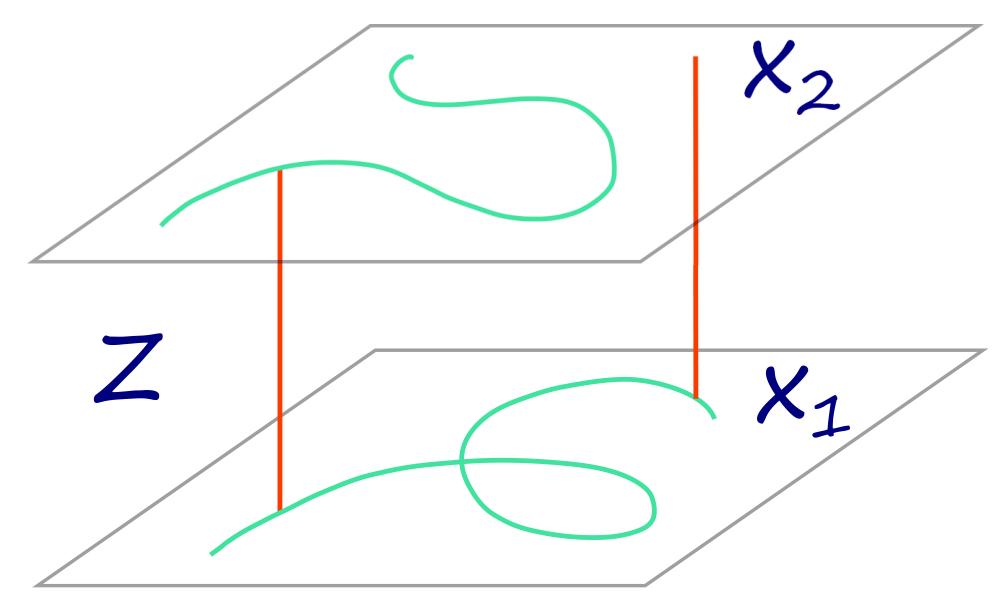
\includegraphics[width=0.62\textwidth]{figures/fig1_connectors.png}
 \caption{$\Cq$-不动点轨迹 $X$ 可以是不连通的，映射 $\pi_{\MM}$ 保留位于 $X$ 中的 $\Cq$-不变曲线的那些分支，而丢弃图中竖直画出的 $\Cq$-轨道。}
  \label{f_connectors}
\end{figure}

\subsubsection{\ }

考虑映射图
$$
\begin{tikzcd}[column sep=large,row sep=large]
\MM(Z) & \MM(Z)^{\Cq} \arrow[l, "\displaystyle{\iota}"'] \arrow[rd, "\displaystyle{\pi_{\MM}}"'] \\
& & \PT(X) \arrow[ld, "\displaystyle{\pi_{\PT}}"'] \\
& \Chow(X)
\end{tikzcd}
$$
其中 $\iota$ 是不动点轨迹的包含映射。假设可以为 $\tO_{\MM}$ 证明一个等变局部化公式，它将在不动点轨迹上产生一个层 $\tO_{\MM,\textup{localized}}$，使得
$$
\iota_* \tO_{\MM,\textup{localized}} =  \tO_{\MM}
$$
在 $\MM(Z)$ 的局部化等变 $K$-理论中成立。我们记
$$
 \tO_{\MM,\textup{localized}} = \iota_*^{-1} \,  \tO_{\MM} \,.
$$
这使我们能够比较 $\tO_{\MM,\textup{localized}}$ 前推到 $X$ 的 Chow 簇与层一侧类似的前推。

\subsubsection{\ }
存在自然的 $S(d)$-不变映射
$$
\Sigma_d: \Chow(X)^{\times d} \to \Chow(X)
$$
由循环的加法给出
$$
\left(\cC_1,\dots,\cC_d\right) \mapsto \sum \cC_i \,.
$$
给定 $\Chow(X)$ 上的一个层 $\cF$，我们定义它在 $\Chow(X)$ 上的对称代数为
$$
\bS_{\Chow}\,  \cF = \bigoplus_{d=0}^{\infty} \left( \Sigma_{d,*} \cF^{\boxtimes d}
\right)^{S(d)} \,.
$$

\subsubsection{\ }

以下是我们的主要猜想，以抽象形式表述：

\begin{Conjecture}\label{sconj1} 在 Chow 簇的 $\TK(Z) \times G_q$-等变 $K$-理论中，我们有如下等式：
\begin{equation}
\bS_{\Chow}\,  \pi_{\MM,*} \, \iota_*^{-1} \, \tO_{\MM} = \pi_{\PT,*} \,
\left(
\tO_{\PT} \otimes \bPhi \right)\label{conj1}
\end{equation}
其中 $\bPhi$ 是 $\prod \PT(X_i)$ 上通用层的某个显式组合，描述 $X$ 的各分支在 $Z$ 内部的相互作用，见下面的第 \ref{s_inter} 节。
\end{Conjecture}

修正的虚拟结构层 $\tO_{\MM}$ 和 $\tO_{\PT}$ 分别在第 \ref{s_DT} 节和第 \ref{s_M} 节中讨论。相互作用项 $\bPhi$ 显式依赖于变量 $Q^{[C_i]} \in \Rep \TK(Z)$，其中 $C_i$ 是被映射 $\pi_{\MM}$ 丢弃的 $\Cq$-不变曲线。

\subsubsection{\ }

把我们的猜想表述为 Chow 簇上层的比较有许多优点。

最重要的是，在本文中我们只在构造层 $\tO_{\MM}$ 方面取得了部分进展。然而，在 Chow 簇的一个大的开集上对它有很好的理解，并且相应的陈述 \eqref{conj1} 是非常非平凡的，可以经受许多检验。

此外，构造修正的虚拟结构层 $\tO_{\MM}$ 和 $\tO_{\PT}$ 需要找到某些线丛的平方根。为了使这些平方根全局存在，可能需要引入一个由从 Chow 簇拉回的线丛给出的额外扭曲，见第 \ref{pull_square} 节。表述 \eqref{conj1} 在一个技术性条件\footnote{原则上，可能发生这样的情况：被映射 $\pi_{\MM}$ \emph{丢弃}的 $\Cq$-轨道的模空间不承认虚拟典范丛的平方根，见第 \ref{s_23inter} 节的讨论。}下避免了这些复杂性。

\subsection{11 维超引力的场与零次数 DT 计数}

\subsubsection{\ }

M-理论是一个量子引力理论，人们相信它在低能下约化为十一维超引力。

在本文中，我们主要关注膜对 M-理论指标的贡献。超引力场对指标也有贡献，原则上它因其局部性质而更容易确定。场指标与零次数 $K$-理论 Donaldson-Thomas 不变量之间的推测联系在 \cite{Zth, ZthJ} 中被发现。由于本文是 \cite{Zth} 思想的自然发展，我们在此简要总结它们。

\subsubsection{\ }

我们在 Hamiltonian 形式下考虑形如 \eqref{eSZ} 的流形上的 M-理论，并围绕某个真空构型线性化。这意味着我们把构型空间取为
$$
\Conf = \frac{\{ \textup{$Z$ 上玻色子场的全局截面}\}}
{\textup{规范等价}  \sim} \,,
$$
其中十一维超引力的线性化玻色子场是某个背景度量 $g_0$ 的小扰动
$$
{\delta}g \in \Gamma(S^2 T^*Z) \,,
$$
以及 $3$-形式
$$
A \in \Gamma(\Omega^3 Z) \,.
$$
在线性化层面，规范等价类就是由 $Z$ 上的向量场和 $2$-形式的像给出的陪集，它们分别通过无穷小微分同胚和
$$
A \mapsto A + d \omega\,, \quad \omega \in \Gamma(\Omega^2 Z)\,,
$$
起作用。特别地，$\Conf$ 是一个无穷维线性空间（即使对紧致 $Z$ 也是如此，因为此时截面和丛都不是全纯的）。此外，在正则引力中，人们还施加十一维时空流形微分同胚下的不变性。在施加 Diff$(Z)$ 不变性之后，还有一个约束，即所谓的 Hamiltonian 约束，它是 $\Conf$ 上适当线丛的允许截面所必须满足的一个二阶微分-变分方程。我们不去试图求解这个约束，而是为了枚举解的目的，限制度量扰动的类别就足够了。一个方便的选择是对 ${\delta}g$ 施加无迹约束：
$$
{\tr} g_{0}^{-1}{\delta}g = 0
$$
其中我们用背景度量 $g_0$ 把 $g_{0}^{-1}{\delta}g$ 变成一个算子 $g_{0}^{-1}{\delta}g : TZ \mapsto TZ$。

$g_0$ 的等距同构通过线性算子作用在 $\Conf$ 上。

\subsubsection{\ }

虽然截面的正则性问题、边界条件等在物理上极其重要，但指标计算通常对这些问题不太敏感，在目前的讨论中我们将完全忽略它们。我们的计算将形式上以下面的基本例子为模型。

假设 $\Conf$ 是一个有限维实向量空间，带有一个紧群 $G$ 的线性作用。特别地，作为 $G$-模有 $\Conf\cong \Conf^*$。令 $\mu$ 为 $\Conf$ 上总是存在的 $G$-不变测度。我们可以找到一个增长的 $G$-不变函数 $f(x)$，使得映射
\begin{equation}
  \label{poly_to_functions}
   \Sd \Conf \otimes_{\R} \C \owns p(x) \mapsto p(x) e^{-f(x)} \in L^2(\Conf,\mu)
\end{equation}
具有稠密的像。由于重数无穷，\eqref{poly_to_functions} 的任何一边都没有良定义的 $G$-特征，但多项式上的次数分级允许构造如下级数
$$
\sum_{k\ge 0}  t^k \, \tr_{\bS^k \Conf} g  = \exp\left( \sum_{n\ge 1} \frac{t^n}{n}
\, \tr_{\Conf} g^n \right)\,, \quad g\in G\,,
$$
它将代替我们充当 $L^2(\Conf,\mu)$ 的 $G$-特征。

\subsubsection{\ }

奇数自由度是
\begin{equation}
\Psi \oplus \Psi^* = \{ \textup{$Z$ 上费米子场的全局截面}\}
\Big/ \sim \,,
\label{odd_conf}
\end{equation}
其中 M-理论的费米子场是自旋 $3/2$ 的 Rarita-Schwinger 场 $\psi_{\pm}$。它们在群 $Spin(V)$ 的表示
$$
V^{3/2}_{\pm} = \Ker \left( V \otimes S_{\pm} \to S_{\mp} \right)
$$
中变换，其中
$$
V=T_{z_0} Z \cong \R^{10}\,,
$$
而 $S_{\pm}$ 是 $Spin(V)$（即 $SO(V)$ 的双重覆盖）的旋量表示。规范变换的 Lie 代数也扩展为包括变换
$$
\psi \mapsto \psi + \nabla \textup{spinor}  \,,
$$
它使 $\psi$ 增加旋量场的一个导数。如果我们围绕 RS 场消失处线性化，那么构型超空间是它的偶子空间和奇子空间的直积。

\subsubsection{\ }

构造空间 $L^2(\Conf,\Ld \Psi^*)$ 需要在 \eqref{odd_conf} 中选择一个极化。一个重要的点（下面会再次讨论）是，两个自然选择
$$
\Psi^* = \{ \textup{$Z$ 上的全局 $\psi_{\pm}$} \}
$$
给出对偶且\emph{不等价}的答案。目前，我们固定一个选择，即 $\psi_+$。那么 $L^2(\Conf,\Ld
\Psi^*)$ 的 $\Iso(g_0)$-指标是以下虚丛的全局截面的对称代数
\begin{alignat}{2}
\underline{\mathit{Conf}_{\textup{super}}} = & S^2 T Z - 1 &\qquad & \textup{无迹度量}  \label{Conf_bundle}\\
& - TZ &\qquad & \textup{模掉微分同胚} \notag \\
 & \Omega^3 Z - \Omega^2 Z + \Omega^1 Z - 1 &\qquad & \textup{$3$-形式模掉正合形式} \notag \\
& -TZ\otimes S_+ + S_+ + S_- &\qquad & \textup{RS 场模掉正合形式}
\notag
\,.
 \end{alignat}

\subsubsection{\ }

现在假设 $g_0$ 是一个 Kähler 度量，并选择 $G\subset
\Iso(g_0)$ 使其在平凡丛 $\Omega^{5,0} Z$ 上平凡作用。那么作为 $G$-丛
$$
S_{\pm} = \Lambda^{\textup{even/odd}} T^{1,0} Z
$$
直接用特征计算证明了以下关键的

\begin{Proposition}[\cite{Zth}] 对如上所述的 $G$，我们有
$$
\underline{\mathit{Conf}_{\textup{super}}} = - T^{1,0}
\otimes(S_{+}-S_{-})
$$
作为 $G$-丛，因此由 Dolbeault 定理，
$$
L^2(\Conf, \Ld\Psi^*) = \Ld
\chi (TZ)  \,,
$$
作为虚 $G$-模，其中 $\chi$ 是全纯 Euler 示性数。
\end{Proposition}

\noindent
注意，交换 $S_+$ 和 $S_-$ 的角色会把答案变为
$$
 \overline{\Ld
\chi  (TZ)} =
\Sd \chi (T^*Z)\,.
$$
\cite{Zth} 中关于零次数 DT 不变量的推测公式，经过适当解释，是\emph{两个}答案的乘积，即 $\Sd \chi (T^*Z-TZ)$，见下面的猜想 \ref{c_DT0}。

对这种加倍现象有一个好的解释将很有趣，它可以与 3-重流形的同调 Gromov-Witten 和 Donaldson-Thomas 不变量对应中零次数部分发生的平方现象相比较 \cite{mnop}。本文不再进一步讨论它，读者可参阅原始论文 \cite{Zth} 获取更多信息。

\subsubsection{\ }
假设 $Z$ 是三重流形 $X$ 上两个线丛 $\cL_1$ 和 $\cL_2$ 的全空间，且 $\cL_1 \otimes \cL_2 = \cK_X$。那么由局部化，
$$
\chi(Z,TZ) = \chi
\left(X,\frac{TZ\big|_X}{(1-\cL_1^{-1}) (1-\cL_2^{-1})}\right)
$$
并且进一步
\begin{multline}
  \frac{T^*Z\big|_X- TZ\big|_X}{(1-\cL_1^{-1}) (1-\cL_2^{-1})} =\cK_X
  - \cO_X + \\
  \frac{\cL_1}{(1-\cL_1) (1-\cL_2^{-1})}
\left( TX + \cK_X - T^*X- \cK_X^*\right) \label{deg0class1} \,.
  \end{multline}
现在注意，若 $\Cq$ 分别以权重 $q$ 和 $q^{-1}$ 作用在 $\cL_1$ 和 $\cL_2$ 上，则 \eqref{deg0class1} 第二行中出现的所有权重都是正的，因此该项的对称代数在 $\Cq$-等变 $K$-理论中是良定义的。把 \eqref{deg0class1} 右端第一项的贡献看作一个（可能无穷的）前因子而不计，我们就接触到 \cite{Zth} 中一个猜想的如下重述。

\subsubsection{\ }
令
$$
\Hilb(X,\textup{points}) = \bigsqcup_{n\ge 0} \Hilb(X,n)
$$
为 $X$ 的点 Hilbert 概形，并考虑其上的如下层
$$
\tO_{\textup{vir}} = (-q)^{\chi(\cO/\cI)} \, \Ovir \otimes
\left(\Kvir \otimes \det
H^0(\cO/\cI \otimes(\cL_1-\cL_2))\right)^{1/2}
$$
其中 $\cO/\cI$ 是 $X$ 的通用 $0$ 维子概形的结构层。这是下面定义和讨论的层 $\tO_{\textup{vir}}$ 的一个特例，所以我们这里不再进一步讨论它。

\begin{Conjecture}[\cite{Zth}]\label{c_DT0} 对如上所述的 $X$
$$
\chi\left(\Hilb(X,\textup{points}),\tO_{\textup{vir}}\right) =
\Sd \chi\left(X,\frac{q \cL_1 \left( TX + \cK_X - T^*X- \cK_X^*\right)}{(1-q\cL_1) (1-q\cL_2^{-1})}
\right)
$$
\end{Conjecture}

我们期待推测的 PT/DT 对应 \cite{PT} 按如下方式推广到 $K$-理论不变量
\begin{equation}
  \label{ePTDT}
  \chi\left(\PT(X),\tO_{\textup{vir}}\right)  \overset?=
\frac{\chi\left(\Hilb(X,\textup{curves}),\tO_{\textup{vir}}\right)}
{\chi\left(\Hilb(X,\textup{points}),\tO_{\textup{vir}}\right)} \,.
\end{equation}

\subsubsection{\ }
为了具体理解这意味着什么，取 $Z=\C^5$，令 $t_1,\dots,t_5$ 为坐标方向的权重。它们满足
\begin{equation}
  \label{prodt}
\prod t_i =1 \,.
\end{equation}
我们有
$$
\chi(Z,TZ^*) = \frac{\sum_1^5 t_i^{-1}}{\prod_1^5 (1-t_i^{-1})} \,,
$$
其中分母可以利用 \eqref{prodt} 对称化。恒等式 \eqref{deg0class1} 表明
\begin{multline}
\frac{\sum_1^5 t_i^{-1}-\sum_1^5 t_i}{\prod_1^5 (t_i^{1/2}-t_i^{-1/2})}
= \\
\frac{-(t_1 t_2 t_3)^{1/2}+(t_1 t_2 t_3)^{-1/2}}
{\prod_1^3 (t_i^{1/2}-t_i^{-1/2})} \, +
\frac{\prod_{i<j\le 3}  \left((t_i t_j)^{1/2}-(t_i t_j)^{-1/2}\right)}
{\prod_1^5 (t_i^{1/2}-t_i^{-1/2})}\label{id0cl}
\end{multline}
只要 \eqref{prodt} 成立。

\eqref{id0cl} 左端的第一项不涉及 $t_4$ 或 $t_5$，可以看作对 Hilbert 概形上积分的微扰贡献。\eqref{id0cl} 左端的第二项（我们记为 $F(t)$，其中已经可以看出 $1$ 个点 Hilbert 概形的贡献）如下计算零次数 DT 不变量。

丛 $\cL_1$ 和 $\cL_2$ 是平凡丛，权重分别为 $t_4$ 和 $t_5$。因此在 $n$ 个点的 Hilbert 概形 $\Hilb(\C^3,n)$ 上，线丛 $\det H^0(\cO/\cI \otimes(\cL_1-\cL_2))$ 是平凡的，权重为 $(t_4/t_5)^n=q^{2n}$。因此，猜想 \ref{c_DT0} 意味着
$$
\sum_{n\ge 0} (-q)^n \chi\left(\Hilb(\C^3,n), \Ovir \otimes
\Kvir^{1/2}\right) \overset?=
\exp \left( \sum_{n=1}^{\infty} \frac{F(t^n)}{n} \right)
$$
其中
$$
t_4 = q^{1/2} (t_1 t_2 t_3)^{-1/2} \,, \quad
t_5 = q^{-1/2} (t_1 t_2 t_3)^{-1/2} \,.
$$
\eqref{id0cl} 右端具有完全的 $5$ 维对称性，这一事实是对 M-理论范式的一个非常非平凡的确认。
\section{DT 被积函数}\label{s_DT}

\subsection{修正的虚拟结构层}

\subsubsection{\ }

$X$ 的 DT 模空间在其最初的定义 \cite{Thom} 中，参数化 $X$ 中一维子概形的理想层 $\cI \subset \cO_X$。它们具有由
\begin{align}
\Def - \Obs &= \chi(\cO_X) - \chi(\cI,\cI) \label{defI}
\\
 &= \chi(\cF) + \chi(\cF,\cO_X) - \chi(\cF,\cF) \notag\,,
\end{align}
描述的完美障碍理论，其中 $\cF = \cO/\cI$ 是 $X$ 上通用的一维层。

$X$ 上层复形的其他稳定性条件给出替代的 DT 模空间。特别地，在 Pandharipande-Thomas 腔室 \cite{PT} 中，模空间参数化配对
$$
s: \cO_X \to \cF
$$
其中 $\cF$ 是纯一维层，且截面 $s$ 的余核具有有限长度。它们的障碍理论的 $K$-理论类的公式是相同的。

\subsubsection{\ }

完美障碍理论以通常的方式（见例如 \cite{FG}）定义虚拟结构层 $\Ovir$。例如，若 $p\in \PT(X)$ 是环面 $\bT$ 的一个孤立不动点，且
$$
\Def_p - \Obs_p = \sum a_i - \sum b_i \,, \quad a_i,b_j \in \bT^{\vee}\,,
$$
是 $p$ 处形变理论的特征，则 $\Ovir$ 在 $p$ 处的局部化（在 $\bT$-等变 $K$-理论中）等于
\begin{equation}
\cO_{\textup{vir},\textup{localized}} =
\frac{\prod \left(1-b_i^{-1}\right)}
{\prod \left(1-a_i^{-1}\right)}  \,.
\label{locOvir}
\end{equation}

\subsubsection{\ }

虚拟典范丛定义为
$$
\Kvir = \frac{\det \Obs}{\det \Def} \,.
$$
对我们特别重要的是它的平方根 $\Kvir^{1/2}$，与第 \ref{s_Spinor} 节比较。

平方根的不同选择（由 Picard 群中的 $2$-挠元联系）对应于理论中费米子的不同边界条件。这意味着它们定义了理论的不同扇区，在具体计算中必须相互匹配。

若 $p$ 是如 \eqref{locOvir} 中的孤立不动点，则
\begin{equation}
\left(\Ovir \otimes \Kvir^{1/2} \right)_{\textup{localized}} =
\frac{\prod \left(b_i^{1/2}-b_i^{-1/2}
\right)}{\prod \left(a_i^{1/2}-a_i^{-1/2}\right)}  \,.
\label{locKvir}
\end{equation}

\subsubsection{\ }\label{s_Hodge}
由 $\Kvir^{1/2}$ 的扭曲使 K-理论 DT 计算大大接近人们熟悉的层上同调问题。

在 DT 理论中，形变与障碍之间存在某种程度的对偶性，当 $\cK_X$ 限制到 $\cF$ 的支集上为平凡丛时具有完美的对偶性。因此，记住下面这个自对偶障碍理论的婴儿例子是有用的，我们下面会再次回到它。

设 $M$ 是一个光滑代数簇，看作其余切丛的零截面
$$
s: M \to T^*M
$$
相应的障碍理论是
$$
\Def - \Obs = TM - T^*M
$$
其中
$$
\Ovir = s^*(\cO_M) = \sum_{k=0}^{\dim M} (-1)^k \Lambda^k TM \,.
$$
我们有
$$
\Kvir^{1/2} = \cK_M
$$
因此
\begin{equation}
\Ovir \otimes \Kvir^{1/2} = (-1)^{\dim M}
\sum_{k=0}^{\dim M} (-1)^k \, \Omega^k M \,.
\label{OvirOmega}
\end{equation}
如果环面以权重 $t$ 缩放 $T^*M$ 的纤维，那么它以权重 $t^{k-\dim M/2}$ 缩放 \eqref{OvirOmega} 中的 $\Omega^k M$ 项。因此
$$
\chi \left(\Ovir \otimes \Kvir^{1/2}\right) =
\sum_{p,q} (-1)^{p-\dim/2} (-t)^{q-\dim/2} H^p(\Omega^q M)
$$
是 $M$ 的中心化 Hodge 多项式的一个特化。

\subsubsection{\ }

$X$ 上的一个层 $\cG$ 给出 DT 模空间上的一个线丛
$$
\bL_{\cG}
= \det H^*(X,\cF \otimes \cG)
$$
其中 $\cF$ 是通用一维层，例如在 Hilbert 概形腔室中 $\cF = \cO/\cI$。

\subsubsection{\ }

如果 $\cG$ 是一维的，那么 $\bL_{\cG}$ 的次数可以如下计算。设 $B$ 是层的一维族，令 $\cF$ 表示 $B \times X$ 上相应的层。令
$$
p_X: B \times X \to X
$$
表示投影，并令
$$
\sweep(B) = p_X \left(\cycle(\cF)\right)
$$
表示 $B$ 中层的循环所扫过的 $X$ 中的 $2$-循环。由 Grothendieck-Riemann-Roch，我们有
\begin{equation}
\deg_{B} \bL_{\cG} = \sweep(B) \, \cdot \, \cycle(\cG) \,.
\label{degbL}
\end{equation}
注意，扫过平凡的族恰好是被到 Chow 簇的映射收缩的那些族，事实上可以证明 \cite{JO} 丛 $\bL_{\cG}$ 是从 Chow 簇拉回的。

\subsubsection{\ }

对称地，对于一维的 $\cG$，丛 $\bL_{\cG}\in \Pic \DT(X)$ 只依赖于 $\cycle(\cG)$，事实上只依赖于它的有理等价类。

\subsubsection{\ }

现在我们已经为修正的虚拟结构层 $\tO_{\DT}$ 的定义准备好了一切要素。

设 $X$ 是如上所述 $\Cq$ 作用在非奇异 Calabi-Yau 五重流形 $Z$ 上的不动点轨迹。由于 $\Cq$ 保持全纯 $5$-形式 $\Omega^5$，我们有
$$
N_{X} Z = \cL_1 \oplus \cL_2
$$
其中 $\Cq$ 分别以权重 $q$ 和 $q^{-1}$ 作用。$\cK_Z$ 的平凡性蕴含
$$
\cL_1 \otimes \cL_2 = \cK_X \,.
$$
线丛 $\cL_1$ 和 $\cL_2$ 的角色将\emph{不}是对称的，反映了第 \ref{coneCq} 节强调的选择：$\cL_1$ 方向在 $q\to 0$ 时是吸引的，而 $\cL_2$ 方向是排斥的。

给定 $X$ 上的一维层 $\cF$，我们用
$$
\chi = \chi(\cF)\,, \quad \beta = \left[\cycle(\cF)\right] \in H_2(X,\Z)
$$
表示它的离散不变量。DT 模空间在对应于 $\cF$ 的点处的虚拟维数等于
$$
\textup{vir dim} = - (\cK_X,\beta) = - (\cL_1+\cL_2,\beta) \,.
$$
\begin{Definition}
我们定义
\begin{equation}
  \label{deftODT}
  \tO_{\DT} = \textup{前因子}  \, \,
 \Ovir \otimes \left( \Kvir \otimes \bL_{\cL_1-\cL_2} \right)^{1/2}
\end{equation}
其中
\begin{align}
  \label{deftODT2}
  \textup{前因子} &=
(-1)^{\frac{(\cL_1-\cL_2,\beta)}{2}} \, (-q)^{-\frac{\textup{vir dim}}2+\chi} \,
Q^{\beta} \\
&= 
(-1)^{(\cL_1,\beta)+\chi} \, q^{-\frac{\textup{vir dim}}2+\chi} \,
Q^{\beta} \notag \,.
\end{align}
\end{Definition}
注意在 $\bL_{\cL_1-\cL_2}$ 项中我们有 $K$-类的差，而不是比 $\cL_1 \otimes \cL_2^{-1} \in \Pic(X)$。对这种形式的 DT 被积函数有一个简单的解释，见第 \ref{s_lowest_term} 节。

我们将在第 \ref{pull_square} 节看到
$$
\Kvir \otimes \bL_{\cL_1-\cL_2} = \textup{square} \otimes
\bL_{c_1(\cL_1) \cap
c_1(\cL_2)}\,,
$$
其中第二个因子如前面的讨论那样是从 $X$ 的 Chow 簇拉回的。

\subsection{相互作用项 $\bPhi$}

\subsubsection{$A_{r-1}$ 曲面纤维化}\label{sAr}

为了讨论 $Z^{\Cq}$ 不同分支之间的相互作用，记住下面最简单的例子是方便的。令
$$
Z_1 =
\begin{matrix}
\cL_1 \oplus \cL_2  \\
\downarrow\\
X
\end{matrix} \,, \quad \cL_1 \otimes \cL_2 = \cK_X \,,
$$
为 $X$ 上两个线丛的全空间。令 $\Cq$ 通过 $\textup{diag}(q,q^{-1})$ 缩放纤维，令 $\mu_r\subset \Cq$ 为 $r$ 次单位根群。令
$$
\begin{tikzcd}[row sep=small,column sep=large]
A_{r-1} \arrow[r,hook] & Z_r \arrow[d] \\
& X
\end{tikzcd}
$$
为商 $Z_1\big/\mu_r$ 的最小解消。它在 $X$ 上纤维化为 $A_{r-1}$-曲面
$$
A_{r-1} = \widetilde{\C^2/\mu_r}\,,
$$
即奇点 $x^{r} = yz$ 的最小解消。在
$$
1 \to \mu_r \to \Cq \xrightarrow{\,\,\,
 q\mapsto q^r \, } \Ct_{q^r} \to 1
$$
中的商以典范方式作用在 $Z_r$ 上，且
$$
Z_r^{\Ct_{q^r}} = X \times \{ \textup{$r$ 个点}\}  \,.
$$
在这个例子中，我们将看到 $X$ 上秩 $r$ 的 Donaldson-Thomas 理论从 $r$ 个 $X$ 副本上秩 $1$ 理论的相互作用中出现，见第 \ref{eng_Hr} 节。

\subsubsection{未断裂的曲线}

回到一般情形，设 $C\subset Z$ 是一条约化连通的 $\Cq$-不变曲线。若 $\Cq$ 在 $C$ 的每个分支上非平凡作用，我们称 $C$ 是\emph{未断裂的}。这意味着 $C$ 是有理的，至多有结点，并且结点处的两个分支具有相反的权重。这也意味着它有两个非奇异不动点 $p_1,p_2 \in C$，它们位于不动点轨迹的两个不同分支 $X_1$ 和 $X_2$ 上。若 $T_{p_1} C$ 的 $\Cq$-权重为正，我们称 $C$\emph{从 $X_2$ 流向 $X_1$}。我们用 $\cU_{21}$ 表示从 $X_2$ 到 $X_1$ 的未断裂曲线的模空间。

由于两个空间 $T_{p_i} Z$ 都有三个平凡的 $\Cq$-权重，$C$ 的法丛有两种可能，即作为 $\Cq$-等变层
\begin{equation}
N_C Z =
\begin{cases}
\cO(-p_1-p_2) \oplus \cO^{\oplus 3}\,, &\textup{或者}\\
\cO(-p_1) \oplus \cO(-p_2) \oplus \cO^{\oplus 2} \,,
\end{cases}\label{NCcases}
\end{equation}
在 \eqref{NCcases} 的第一种情形中，
$$
\cU_{21} \cong X_1 \cong X_2
$$
带有障碍丛
$$
H^1(C,\cO(-p_1-p_2)) \cong \cL_1\big|_{p_i} \otimes \cL_2\big|_{p_i}
\cong
\cK_{X_i} \big|_{p_i} \quad i=1,2 \,,
$$
其中像通常一样，我们用 $\cL_1$ 和 $\cL_2$ 表示不动点轨迹法丛中的 $\Cq$-特征丛。在 \eqref{NCcases} 的第二种情形中，形变是二维且无阻碍的。未断裂曲线的模空间
$$
X_2 \hookleftarrow \cU_{21} \hookrightarrow X_1
$$
作为光滑曲面嵌入每个 $X_i$ 中。

\subsubsection{三重流形与曲面相互作用}\label{s_23inter}

我们把 \eqref{NCcases} 中的两种情形分别称为三重流形相互作用和曲面相互作用。例如，在第 \ref{sAr} 节的例子中，任意一对不动分支之间都存在三重流形相互作用。相应的未断裂曲线是 $A_{r-1}$ 纤维中的 $(-2)$-曲线。

曲面相互作用的例子可以如下构造。取
$$
Y =
\begin{matrix}
\cO(-1)\oplus \cO(-1) \\
\downarrow\\
\pP^1
\end{matrix}
$$
并使 $\Cq$ 通过缩放基 $\pP^1$ 作用在 $Y$ 上，使得在每个不动点上方的纤维中有一个平凡权重。除了 $Y$，我们还可以取许多其他包含具有 $\cO(-1)\oplus \cO(-1)$ 法丛的 $\Cq$-不变曲线的环面 CY 三重流形。考虑与一个主 $(\Ct)^3$-丛 $P$ 相关联的曲面 $S$ 上的 $Y$-丛
$$
Z = P \times_{(\Ct)^3} Y\,, \quad c_1(P) = \cK_S
$$
我们看到 $\cK_Z \cong \cO_Z$，$X_1$ 和 $X_2$ 是 $S$ 上的线丛，且
$$
\cU_{21} \cong S
$$
作为零截面嵌入它们每一个中。由于曲面 $S$ 是任意的，我们得出 $\cK_{\cU_{21}}$ 可能不是平方。

\subsubsection{算子 $\Phi_{ij}$}

障碍理论
$$
\Def - \Obs = H^*(C,N_C Z)
$$
给 $\cU_{21}$ 一个虚拟维数为 $2$ 的虚拟结构层。对于三重流形相互作用，相应的虚拟典范丛总是平方，其中
$$
\tO_{\cU_{21}} = \cK_{X_i}- \cO_{X_i} \,.
$$
对于曲面相互作用，我们\emph{假设}
$$
\tO_{\cU_{21}}  = \cK^{1/2}_{\cU_{21}}
$$
中的平方根存在，并在任一情形下定义
$$
\Phi_{21} = \eval_*  \tO_{\cU_{21}} \,,
$$
其中
$$
\eval: \cU_{21} \to X_2 \times X_1
$$
把一条未断裂曲线 $C$ 送到不动点 $(p_2,p_1)$。我们用同一个符号 $\Phi_{21}$ 表示相应的 Fourier-Mukai 算子
$$
\cF_1 \xrightarrow{\,\,\Phi_{21}\,\,} p_{X_2,*}
\left(\Phi_{21} \otimes
p_{X_1}^* \, \cF_1 \right) \,.
$$
例如，对于三重流形相互作用
$$
\Phi_{21} \, \cF_1 = \cK_X \otimes \cF_1 - \cF_1 \,.
$$

\subsubsection{相互作用}\label{s_inter}

设 $X_1$ 和 $X_2$ 是如上所述的 $X$ 的两个分支，令 $\cF_1$ 和 $\cF_2$ 表示 $X_1$ 和 $X_2$ 的 DT 模空间上的通用一维层。利用算子 $\Phi_{21}$，我们可以定义如下 $K$-理论类
\begin{equation}
\cX_{21} = \chi(\cO_{X_2}-\cF_2, \Phi_{21} (\cO_{X_1}-\cF_1)) \label{defX21}
\end{equation}
它可以与 DT 模空间虚拟切空间的公式 \eqref{defI} 相比较。

我们定义
\begin{equation}
\bPhi = \bigotimes_{i<j} \bS \, Q^{[C_{ij}]} \, \cX_{ji}\,,
\label{defbPhi}
\end{equation}
其中 $S$ 表示对称代数，
$$
[C_{ij}] \in H_2(Z,\Z)
$$
是从 $X_j$ 流向 $X_i$ 的未断裂曲线的类，各分支的编号使得曲线从较大的分支流向较小的分支。

\subsubsection{一个例子}

对于三重流形相互作用，利用 Serre 对偶我们有
\begin{equation}
  \cX_{21} = -
\chi(\cI_2,\cI_1) - \overline{\chi(\cI_1,\cI_2)} \label{XA}
\end{equation}
其中 $[\cI]=[\cO_X] - [\cF]$，横线表示对偶。这样的相互作用项自然出现在高秩 DT 理论中，见下面的第 \ref{e_rank} 节。

\subsubsection{微扰贡献}\label{s_pert}

注意，若 $X_i$ 不是固有的，Euler 示性数 \eqref{defX21} 可能不是良定义的。然而，差
\begin{multline}
 \cX'_{21}= \cX_{21} - \chi(\cO_{X_2},\Phi_{21} \cO_{X_1}) =\\
 -\chi(\cF_2,\Phi_{21} \cO_{X_1})
- \chi(\cO_{X_2},  \Phi_{21}  \cF_1)
 +\chi(\cF_2, \Phi_{21} \cF_1)
\label{X21red}
\end{multline}
是良定义的，并且只与 \eqref{defX21} 相差一个常数（尽管可能是无穷维的）向量空间 $\chi(\cO_{X_2},\Phi_{21}
\cO_{X_1})$。其对称代数的特征
$$
\bS \, Q^{[C_{12}]} \, \chi(\cO_{X_2},\Phi_{21}
\cO_{X_1})
$$
可以用任何传统方法正则化。从 $X$ 上 DT 理论的观点来看，它表现为一个总的前因子，也称为微扰贡献。
\section{膜的指标}\label{s_M}

\subsection{膜的模空间}

\subsubsection{多重曲线}

回想一下，$Z$ 中稳定膜的模空间 $\MM(Z)$ 应该是浸入全纯曲线 $C\subset Z$ 的模空间的某个紧化。这样一个紧化是稳定映射的模空间；也可以考虑使用 $Z$ 上层模空间的紧化。虽然 M2-膜对 M-理论指标的贡献完全有可能用这样的模空间来计算，但本文我们走另一条路线。

处理全纯曲线的主要几何困难在于退化到多重曲线，例如椭圆
$$
y^2 = \lambda (1-x^2)
$$
当 $\lambda\to 0$ 时退化为双重直线 $y^2=0$。物理学家可以把多重曲线称为若干 M2-膜的束缚态。在稳定映射的模空间中，$\lambda\to 0$ 极限是在点 $x=\pm 1$ 处分歧的 $y=0$ 直线的二重覆盖，这些点保留了原椭圆的 $x$-投影的分歧点。在曲线的 Hilbert 概形中，极限将只是平面上由 $y^2=0$ 切出的子概形，不保留原二次曲线的形状。

我们不用 $Z$ 上的层或到 $Z$ 的稳定映射来构造膜模空间的一个原因是，对于给定的次数它们不给出自然的有界模空间，回想第 \ref{Mbound} 节的讨论。例如，在上面的例子中，可能存在 $y=0$ 的具有任意多分歧点的二重覆盖，或者这条直线可能是具有任意大 Euler 示性数的层的支集。

\subsubsection{来自概形的映射}\label{s_mapsf}

在本文中，我们考虑映射
\begin{equation}
f: C \to Z
\label{fCZ}
\end{equation}
其中 $C$ 是一维\emph{概形}。在上述例子中，这就是双重直线的包含映射。一般地，$f$ 不必是单射，例如光滑曲线 $C$ 浸入的情形。

在实际操作中，映射 $f$ 可以表示为某个 $N\gg 0$ 下的子概形
$$
C \subset Z \times \pP^N
$$
其中映射 $f$ 是到第一个因子的投影。利用这种表示，我们定义映射 $f$ 的法层为
$$
N_f = N_C \left(Z \times \pP^N\right) - \cO_C \otimes T \pP^N \,.
$$
这里
$$
N_C \left(Z \times \pP^N\right) = \Hom (\cI_C, \cO_C)\,,
$$
其中 $\cI_C$ 是 $C$ 的理想层，$\cO_C$ 是它的结构层。

当 $C$ 是良态的，例如光滑或局部完全交时，$N_f$ 是一个秩 $4$、次数 $2g-2$ 的向量丛。然而，一般地它可以大得多，反映了映射 \eqref{fCZ} 的模空间的奇异性。下面我们将讨论处理大 $N_f$ 的一些策略。

\subsubsection{稳定性条件}\label{s_stabil}

我们对映射 \eqref{fCZ} 施加如下\emph{稳定性}条件：
\begin{enumerate}
\item[(1)] 映射 $f$ 在 $C$ 中有限个点集之外在其像上是同构。
\item[(2)] 对任意真子概形 $C' \subset C$
\begin{equation}
\frac{\chi(\cO_{\C'})}{\deg f(C')} >
\frac{\chi(\cO_{\C})}{\deg f(C)}
\label{slopestab}
\end{equation}
这意味着 $\chi(\cO_{\C'}) f(C) - \chi(\cO_{\C}) f(C')$ 是 $\supp f(C)$ 各分支的一个非负且非零的线性组合。
\end{enumerate}

\noindent
例如，$\pP^2$ 中的双重直线 $C$ 是稳定的，因为 $\chi(\cO_{\C}) = 1$ 且对 $C$ 的任何子概形有 $\chi(\cO_{\C'}) \ge 1$。

更一般地，设 $C$ 是曲线 $B$ 上线丛 $\cL$ 全空间内的双重零截面。那么
$$
\chi(\cO_C) = 2 \chi(\cO_B) - \deg \cL
$$
因此 \eqref{slopestab} 意味着
$$
\textup{$C$ 稳定} \,\, \Leftrightarrow \,\, \deg \cL > 0 \,.
$$
换句话说，膜只能在法丛的\emph{正方向}上堆叠。

\subsubsection{CM 性质}

一维概形是 Cohen-Macaulay 的，如果对每个点 $x\in C$ 存在一个在 $x$ 处消失且不是零因子的函数 $f$。

如果此条件在某个点 $x\in C$ 处被破坏，那么
$$
\cI_{C'}=\Ann \fm_x \subset \cO_C\,,
$$
其中 $\fm_x$ 是在 $x$ 处消失的函数的理想，是 $\cO_C$ 的一个有限长度的非平凡理想。因此
$$
\cO_{C'} = \cO_{C} / \cI_{C'}
$$
是一个真子概形，满足
$$
\chi(\cO_{C'}) < \chi(\cO_{C})\,, \quad [f(C')] =  [f(C)] \,.
$$
所以，所有稳定映射 \eqref{fCZ} 的源 $C$ 都是 Cohen-Macaulay 的。

从一维 Cohen-Macaulay 概形到射影簇的映射由 H{\o}nsen 在 \cite{Hon} 中研究过，他对于给定的 $\deg f(C)$ 和 $\chi (\cO_C)$ 把它们的模空间构造为一个固有分离的代数空间。他施加了第 \ref{s_stabil} 节中的第一个而非第二个稳定性条件。

\subsubsection{有界性}

对任意映射 \eqref{fCZ}，Euler 示性数 $\chi(\cO_C)$ 可以用 $f(C)$ 的次数\emph{从下方}界定。稳定性 \eqref{slopestab} 也\emph{从上方}界定了它。因此，一旦映射的次数固定，稳定映射 \eqref{fCZ} 形成一个有界族。

这从 M-理论的观点来看是很自然的。在 M-理论中，存在一个 $3$-形式与膜的世界体 $C \times S^1$ 耦合，从而记录它的次数。另一方面，没有场与 $C$ 的 Euler 示性数耦合，而且 $C \times S^1$ 的 Euler 示性数为零，正如任何光滑实三重流形一样。

这意味着在我们猜想的膜一侧，我们对膜的所有 Euler 示性数求和而\emph{不带权}。DT 一侧的 $q^{\chi}$-权重仅仅由于 $\Cq$ 作用而出现，而它的存在是对 $Z$ 的一个额外假设。

\subsection{膜的形变}

\subsubsection{\ }

当法层 $N_f$ 变得太大时，映射 \eqref{fCZ} 的形变理论变得非常复杂和技术化。也许可以从 $f$ 的法复形构造某种形式的虚拟结构层。然而目前，我们计划追求一种更几何的方法，即把 $\MM(Z)$ 取为 H{\o}nsen 空间的某个\emph{虚拟 Nash 吹胀}。

回想一下，奇异空间 $\cM$ 的普通 Nash 吹胀记录了光滑点 $\cM_0 \subset \cM$ 处的切空间在接近奇点时的极限。$\cM$ 的 Nash 吹胀上的一个点由一对 $(p,N)$ 描述，其中 $p\in \cM$ 且
$$
N \subset T_p \cM \,, \quad \dim N = \dim \cM_0 \,.
$$

\subsubsection{\ }

我们假设的 H{\o}nsen 空间的虚拟吹胀 $\MM(Z)$ 应该参数化映射 \eqref{fCZ} 以及一个子层
\begin{equation}
N \subset N_f\label{NinNf}
\end{equation}
它在 $C$ 的 $K$-理论中具有类
$$
[N] = 3 \left[\cO_C\right] + \left[\omega_C \right]
$$
其中 $\omega_C$ 是 Cohen-Macaulay 概形 $C$ 的对偶化层。对 $N$ 的附加条件是目前研究的主题，将单独讨论。

\eqref{NinNf} 中包含的额外数据的一种可能物理解释如下。映射 $f: C\to Z$ 实际上是一个\emph{超概形}映射的玻色子部分，当 $f$ 是浸入或更一般的 l.c.i.\ 映射时，其费米子部分可以唯一重建。当 $f$ 产生奇点时，重建的唯一性失效，而子层 \eqref{NinNf} 存储了缺失的信息。

\subsubsection{\ }

有了这些附加条件，我们希望 $\MM(Z)$ 具有一个障碍理论，使得在 $\MM(Z)$ 的 $K$-理论中
$$
\left[ \Def - \Obs \right] = \left[H^*(N)\right]
$$
我们并不期待这些虚拟丛同构，只期待它们关于某个滤过的部分被等同起来。
\section{例子}
\label{s_exa}

\subsection{约化的局部曲线}\label{s_slc}

\subsubsection{\ }

设 $Z$ 是光滑曲线 $C$ 上四个线丛的全空间
$$
Z =
\begin{matrix}
\cL_1 \oplus \cL_2 \oplus \cL_3 \oplus \cL_4 \\
\downarrow\\
C
\end{matrix} \,, \quad \bigotimes \cL_i = \cK_B \,,
$$
像之前一样，我们令 $\Cq$ 分别以权重 $q$ 和 $q^{-1}$ 作用在 $\cL_1$ 和 $\cL_2$ 上，因此 $X$ 是 $\cL_3\oplus \cL_4$ 的全空间。我们要比较 $Z$ 内零截面 $C$ 的 DT 计数与 M-理论计数。

\subsubsection{\ }

一个三维环面 $\bT$ 通过缩放各个 $\cL_i$ 作用在 $Z$ 上。显然，
$$
\MM(Z,[C])^{\bT} = \{0\}
$$
是一个代表曲线 $C$ 本身的点。我们有
$$
\left(\Def^{\MM}-\Obs^{\MM} \right)\Big|_{0} = H^*(N_C Z) \,, \quad N_C Z =
\bigoplus_{i=1}^4 \cL_i \,.
$$
因此
$$
\chi\left(\MM,\tO_{\textup{vir}}\right) = \left(\det H
\right)^{-1/2}  \Sd  H^{\vee} \,, \quad H=H^*(N_C Z)\,.
$$
实际上，这意味着如果 $\sum a_i - \sum b_i$ 是 $H^*(N_C Z)$ 的特征，则
\begin{equation}
\chi\left(\MM,\tO_{\textup{vir}}\right) =
\prod \frac{b_i^{1/2} -
  b_i^{-1/2} }
{a_i^{1/2} -
  a_i^{-1/2} } \,. \label{prodm}
\end{equation}

\subsubsection{\ }

为了与 DT 理论比较，我们需要把 \eqref{prodm} 按 $q$ 的幂展开。方便起见，把 $\Cq$-运动方向分离出来
$$
N_{12} = \cL_i \oplus \cL_j\,, \quad H_{12} = H^*(N_{12}) \, ,
$$
以及它们对 \eqref{prodm} 的贡献
$$
\chi(\MM,\tO_{\textup{vir}})_{12} = \textup{$N_{12}$ 的贡献}
$$
我们计算
\begin{multline}
\chi(\MM,\tO_{\textup{vir}})_{12}=
(-1)^{h_1} q^{\frac{h_1 + h_2}2} \otimes \\
(\det H^*(\cL_1-\cL_2))^{1/2} \,\,  \Sd \left(q H^*(\cL_1) \oplus
q H^*(\cL_2)^{\vee}\right) \,,
 \label{Minq}
\end{multline}
其中
$$
h_i = \rk H^*(\cL_i) = \deg \cL_i + 1 - g(C) \,.
$$
特别地
\begin{equation}
\chi(\MM,\tO_{\textup{vir}})_{12} =
(-1)^{h_1} q^{\frac{h_1 + h_2}2} \,
(\det H^*(\cL_1-\cL_2))^{1/2} \, (1+O(q)) \,,
 \label{Minql}
\end{equation}
当 $q\to 0$ 时。

\subsubsection{\ }

在 Donaldson-Thomas 一侧，我们有
$$
\PT(X,[C])^{\bT} = \bigsqcup_{n\ge 0} S^n C \,.
$$
这些空间的形变理论由在 $N_{34}$ 方向上形变 $C$ 以及 $S^nC$ 上某个扭曲的余切丛组成，见下文。特别地，$H_{34}$ 对 PT 计数的贡献恰好是 $\chi(\MM,\tO_{\textup{vir}})_{34}$。

回想根据定义 \eqref{deftODT}
$$
\tO_{\DT}  = \textup{前因子}  \, \,
 \Ovir \otimes \left( \Kvir \otimes \det H^*(\cL_1-\cL_2)
 \right)^{1/2}
$$
其中，略去常数项 $Q^C$，
\begin{align}
  \textup{前因子}
&= 
(-1)^{(\cL_1,\beta)+\chi} \, q^{-\frac{\textup{vir dim}}2+\chi} \,
\notag \\
&= 
(-1)^{h_1+n} \, q^{\frac{h_1+h_2}2+n} \,
\label{PTinql}
\end{align}
因为对于由 $S^n C$ 参数化的层 $\cF$ 有 $\chi(\cF)=n+1-g(C)$，且
$$
- \textup{vir dim} = \deg \cK_X = \deg \cL_1 + \deg \cL_2  \,.
$$

\subsubsection{\ }\label{s_lowest_term}

$q$-展开中的最低项对应于 $n=0$。比较 \eqref{Minql} 与 \eqref{PTinql}，我们发现完全一致。事实上，我们看到前因子 \eqref{deftODT2} 的形式是由约化局部曲线的最低 $q$ 项所决定的。

\subsubsection{\ }

对于 $n>0$，$S^n C$ 上有一个非平凡的障碍丛。当 $\cK_X$ 平凡，即
$$
\cL_3 \otimes \cL_4 = \cK_C
$$
时，由形变与障碍之间的对偶性，这是 $S^n C$ 的余切丛。一般地，它是 $T^* S^n C$ 的某个扭曲版本。

令
$$
\Delta \subset S^n C \times C
$$
为通用子概形。回想 \cite{ACGH}
\begin{equation}
T^* S^n C = (p_1)_* \, \cO_{\Delta} \otimes p_2^*(\cK_C)\,,\label{TSn}
\end{equation}
其中 $p_i$ 是到两个因子的投影。更一般地，
$$
\Obs =   (p_1)_* \, \cO_{\Delta} \otimes p_2^*(\cL_3 \otimes \cL_4 )\,.
$$
我们注意到公式
$$
\boxed{\chi\left( \oSd C, \tO_{\DT} \right) = \left(\det H
\right)^{-1/2}  \Sd  H^{\vee}\,,} \qquad H=H^*(\oplus \cL_i )\,,
$$
是 Macdonald 关于曲线的对称幂的 Hodge 数的经典公式的推广。据推测，它有一个初等的证明。

\subsection{双重曲线}

\subsubsection{\ }
设 $\cL$ 是光滑曲线 $B$ 上的线丛，$S_{\cL}$ 是这个线丛的全空间。若 $z$ 是沿 $S_{\cL}$ 纤维的局部坐标，则
$$
\bB_{\cL} = \{z^2=0\} \subset S_{\cL}
$$
是基 $B$ 在纤维方向上的无穷小加厚。我们有
$$
\cO_{\bB_{\cL}} = \cO_{B} \oplus \cL^{-1}
$$
作为 $\cO_B$-模，特别地，
$$
\chi(\bB_{\cL}) = 2 \chi(B) - \deg \cL \,.
$$
$\bB_{\cL}$ 的法丛
$$
N_{\bB_{\cL}} S_{\cL} = \cL \oplus \cL^2
$$
可以具体地看作如下形式的形变
$$
\{ z^2 + p_1 z + p_2 = 0\}\,, \quad p_i \in \Gamma(\cL^i) \,.
$$
一个非常熟悉的例子是双重直线到 $\pP^2$ 中二次曲线的形变，其中法丛没有 $H^1$。

\subsubsection{\ }
设 $D\subset B$ 是次数为 $d$ 的有效除子，令
$$
s_D \in H^0(B,\cO(D))
$$
为重言截面。它定义了一个映射
$$
F_D: S_{\cL(-D)} \owns (b,z) \mapsto (b,s_D(b) z) \in S_{\cL}
$$
其中 $(b,z)$ 是 $F_D$ 定义域中的基坐标和纤维坐标。

映射 $F_D$ 是 $S_{\cL}$ 在子概形 $D\subset
S_{\cL}$ 中的吹胀。它的形变具有形式
$$
\Def(F_D)= T_{D} \Hilb(S_{\cL},d) = T_D \, S^d B + H^0(B,\cO_D
\otimes \cL)
$$
并且它们是无阻碍的。我们已经见过曲线 $B$ 的对称幂 $S^dB$ 的切空间，见 \eqref{TSn}。

\subsubsection{\ }
现在设 $Z$ 是光滑曲线 $B$ 上四个线丛的全空间
$$
Z =
\begin{matrix}
\cL_1 \oplus \cL_2 \oplus \cL_3 \oplus \cL_4 \\
\downarrow\\
B
\end{matrix} \,, \quad \bigotimes \cL_i = \cK_B \,,
$$
让我们在类中寻找 $\bT$-不变的稳定膜
$$
[C] = 2 [B] \,.
$$
这里 $\bT\cong (\Ct)^3$ 是以行列式 $1$ 缩放纤维的环面。

\subsubsection{\ }
我们将作一个简化假设
$$
\deg \cL_1 > 0 \ge \deg \cL_i\,,\quad i=2,3,4 \,,
$$
此时 $C$ 只能如第 \ref{s_stabil} 节所述在 $\cL_1$ 方向上加倍，且所有 $\bT$-不变稳定膜具有形式
\begin{equation}
f_D : \,\, \bB_{\cL_1(-D)}
\hookrightarrow S_{\cL(-D)}
\xrightarrow{\,\,\, F_D \,\,\,} S_{\cL_1} \hookrightarrow Z\,, \label{f_D}
\end{equation}
其中 $D\in S^d B$ 是次数为
$$
0 \le d < \deg \cL_1 \,.
$$
的有效除子。这个范围受稳定性条件 $
\chi\left(\bB_{\cL_1(-D)} \right)< 2  \chi(B)
$ 的约束。

\subsubsection{\ }
映射 \eqref{f_D} 的形变理论可以描述为
$$
\Def(f_D) - \Obs(f_D) = \Def(F_D) + H^*\left(B,N_{\bB_{\cL_1(-D)}} S_{\cL_1(-D)}
+ f_D^* N_{S_{\cL_1}} Z\right)
$$
其中
\begin{align*}
 N_{\bB_{\cL_1(-D)}} S_{\cL_1(-D)}  &= \cL_1(-D) +  \cL_1^2(-2D)\,,\\
f_D^* N_{S_{\cL_1}} Z &= (\cO + \cL_1^{-1}(D)) \otimes (\cL_2
+\cL_3+\cL_4) \,.
\end{align*}

\subsubsection{\ }
当 $B=\pP^1$ 时，相应的膜积分特别容易计算，因为此时可以利用基上的额外环面作用。它们可以与相应的二次 PT 积分比较，后者也可以用局部化计算。像通常一样，事实上不止一个 PT 检验，因为不同的环面可以被指定为 $\Cq$。

\subsection{光滑曲线之间的单次相互作用}

\subsubsection{\ }
设 $X_i$ 是 $X=Z^{\Cq}$ 的分支，令 $C_i \subset X_i$ 是每个分支中光滑约化曲线（可以为空）的集合。如图 \ref{f_connectors} 所示，设 $f: C \to Z$ 是一个 $\Cq$-不变稳定膜，使得
$$
\pi_{\MM} (f(C)) \subset \sum \left[C_i\right]
$$
其中第 \ref{s_pi_DTM} 节的映射 $\pi_{\MM}$ 只保留那些被逐点固定的分支。

我们用 $C'$ 表示 $C$ 的其他分支，这里聚焦于这样一种情形：与图 \ref{f_connectors} 所描绘的情形不同，$C'$ 是从 $p_2 \in X_2$ 流向 $p_1\in X_1$ 的单个 $\Cq$-轨道的闭包。一般情形（$C'$ 可以是可约的或非约化的）预期由 \eqref{defbPhi} 中取对称代数来覆盖。

\subsubsection{\ }
有 $4$ 种可能的情形，即
$$
C =
\begin{cases}
C' \,, \\
C' \cup C_1 \,, \\
C' \cup C_2 \,, \\
C' \cup C_1 \cup C_2 \,,
\end{cases}
$$
对应于 \eqref{defX21} 展开中的 $4$ 个项。我们考虑最后一个、最有趣的情形，假设 $C_1 \ne
\varnothing \ne C_2$。我们用
$$
\Delta N =   N_CZ  - \big(N_{C'}Z + N_{C_1}Z + N_{C_2}Z \big)
$$
表示 $Z$ 的法丛与其各分支的法丛之差。它可以描述为
\begin{align}
\Delta N =  & \,
 T_{p_1} C' \otimes T_{p_1} C_1  + T_{p_2} C' \otimes T_{p_2} C_2
\notag \\
& - T_{p_1} Z + T_{p_1} C' + T_{p_1} C_1 \notag \\
& - T_{p_2} Z + T_{p_2} C' + T_{p_2} C_2 \label{NNC} \,,
\end{align}
其中第一行对应于两个结点的平滑化，而第二行是若 $p_1$ 处的结点未被平滑化时保持该结点的条件。

\subsubsection{\ }
$\Delta N$ 对 $\tO_{\MM}$ 的贡献等于
\begin{align*}
  \left(\det \Delta N \right)^{-1/2} \Sd \Delta N^{\vee} & = \Sd \left( -
    N^{\vee}_{C_1} X_1 \Big|_{p_1}- N_{C_2} X_2 \Big|_{p_2} \right) +
  O(q) \\
&= \eval^*\left(\cO_{C_2}^{\vee} \boxtimes \cO_{C_1} \right) + O(q) \,,
\end{align*}
当 $q\to 0$ 时。于是我们看到，第 \ref{s_inter} 节描述的相互作用形式已经由最简单相互作用几何中的最低 $q$ 项所决定。

\subsection{高秩 DT 计数}\label{e_rank}

\subsubsection{\ }
与 PT 模空间类似，可以考虑带有 $r$ 个截面的一维层 $\cF$，即形如
\begin{equation}
\cO_X^{r} \xrightarrow{\,\,s\,\,} \cF\,,
\label{PTr}
\end{equation}
的复形，满足同样的稳定性条件。它们有一个自然的 $GL(r)$ 作用，通过 $\cO_X^r$ 的自同构实现。

与 $r=1$ 情形相反，当 $r>1$ 时 \eqref{PTr} 的形变一般导致不是 \eqref{PTr} 形式的复形。即使 $X$ 是曲面，这也是一个众所周知的现象：在所有带框架的无挠层 $\cG$ 的模空间中，形如 \eqref{PTr} 的点对应于 $\cG=\Ker s$ 满足 $\cG^{\vee \vee} \cong
\cO_X^r$ 的无挠层，换句话说，对应于零尺寸的瞬子。

\subsubsection{\ }
虽然构造一个包含 \eqref{PTr} 形变的、带 $GL(r)$ 作用的固有模空间当然是一个有许多潜在应用的有趣问题，但这个问题即使对于最简单的曲面 $\C^2$ 目前也仍然开放。

相反，这里我们采取一种实用主义的方法，通过关于最大环面 $\bA\subset GL(r)$ 的局部化来定义高秩 PT 不变量。相应的不动点轨迹是直接和
\begin{equation}
\cO_X^{r} \xrightarrow{\,\,\oplus s_i \,\,} \cF = \bigoplus \cF_i \,,
\label{PTrs}
\end{equation}
因此是 $X$ 的 PT 模空间的 $r$ 重乘积，带有自然的直和障碍理论。为了考虑秩 $r$ 中所需的修改，我们定义
\begin{equation}
  \label{deftODTr}
  \tO_{\DT,r} = \textup{前因子}  \, \,
 \Ovir \otimes \left( \Kvir \otimes \bL^{\otimes r}_{\cL_1-\cL_2}
 \right)^{1/2}
\otimes \textup{交叉项} \,.
\end{equation}
前因子的形式变为
\begin{equation}
  \label{deftODT2r}
  \textup{前因子} =
(-1)^{(r \cL_2 + \cK,\beta)+r \chi} \, q^{(\beta,\cK)+\chi} \,
Q^{\beta} \notag \,,
\end{equation}
其中 $\beta = \ch_2(\cF)$，$\chi=\chi(\cF)$。

\subsubsection{\ }
\eqref{PTrs} 的形变理论中的交叉项按照 $\bA$ 的权重分解，其中项
\begin{equation}
N_{ji} = \chi(\cF_i) + \chi(\cF_j^{\vee}) - \chi(\cF_j,\cF_i) \label{Nji}
\end{equation}
具有权重 $a_i/a_j$。我们有
$$
\textup{交叉项} = \bigotimes_{i\ne j} \tSd N_{ji}
$$
其中对 $K$-理论类 $V$，为简便起见我们令
$$
\tSd V  =\left( \det V \right)^{-1/2} \otimes \Sd V^{\vee}  \,.
$$
第 \ref{pull_square} 节的论证稍作修改即可表明 \eqref{deftODTr} 中的平方根（包括交叉项中出现的平方根）在模掉从 Chow 簇拉回的线丛后是良定义的。

\subsection{构造高秩 DT 理论}\label{eng_Hr}

\subsubsection{\ }
设 $Z_r$ 是如第 \ref{sAr} 节中 $X$ 上的 $A_{r-1}$-曲面纤维化。我们给不动点轨迹的分支编号
$$
Z^{\Cq} = X_1 \sqcup X_2 \sqcup \dots \sqcup X_r
$$
使得未断裂曲线从较大的指标流向较小的指标。在这样的编号下
$$
N_{X_i} Z = \cL_1^{r} \cK^{i-r} \oplus \cL_2^{r} \cK^{1-i} \,, \quad
i=1,\dots, r\,,
$$
其中 $\cK = \cK_X$。按照我们的约定，它们具有 $\Cq$-权重 $(q,q^{-1})$，尽管这里的 $q$ 是在取商与解消之前最初作用在 $Z_1$ 上的变量的 $r$ 次幂。

$Z_r$ 几何的示意表示见图 \ref{f_Z4}。

\subsubsection{\ }
本节的目标是证明以下

\begin{Proposition}\label{p_eng}
在猜想 \ref{sconj1} 下，$Z_r$ 的 M2-膜指标等于 $X$ 的秩 $r$ Donaldson-Thomas 配分函数。
\end{Proposition}

为了使这个陈述有意义，必须用 $GL(r)$-等变参数代替 $Z_r$ 的 Kähler 参数，换句话说，需要一个满射
$$
\gamma: \bA \twoheadrightarrow \TK(Z_r)  \,.
$$
我们从描述 $\gamma$ 开始。

\subsubsection{\ }
为了定义 $\gamma$，只需给出坐标余特征
$$
\delta_i : \Ct \to \bA
$$
在 $\TK(Z_r)$ 的余特征格 $H^2(X,\Z)$ 中的像。

对 $s\in \{\frac12,\frac32,\dots,r+\frac{1}{2}\}$，令
\begin{align*}
D_s &= \textup{$X_{s-1/2}$ 的吸引流形} \\
      &= \textup{$X_{s+1/2}$ 的排斥流形}
\end{align*}
其中吸引和排斥流形是针对 $q\to 0$ 的作用定义的。如图 \ref{f_Z4} 所示。

由构造，这意味着
\begin{equation}
D_s\Big|_{X_i} =
\begin{cases}
c_1(\cL_2^r \cK^{1-i})\,, \quad &i = s-1/2 \,,\\
c_1(\cL_1^r \cK^{i-r})\,, \quad &i = s+1/2 \,, \\
0 \,,  \quad &\textup{其他} \,.
\end{cases}\label{DsX}
\end{equation}
我们令
$$
\gamma(\delta_i) = \frac12 \sum_{s<i} D_s - \frac12 \sum_{s>i} D_s \,.
$$

\begin{figure}[!htbp]
  \centering
   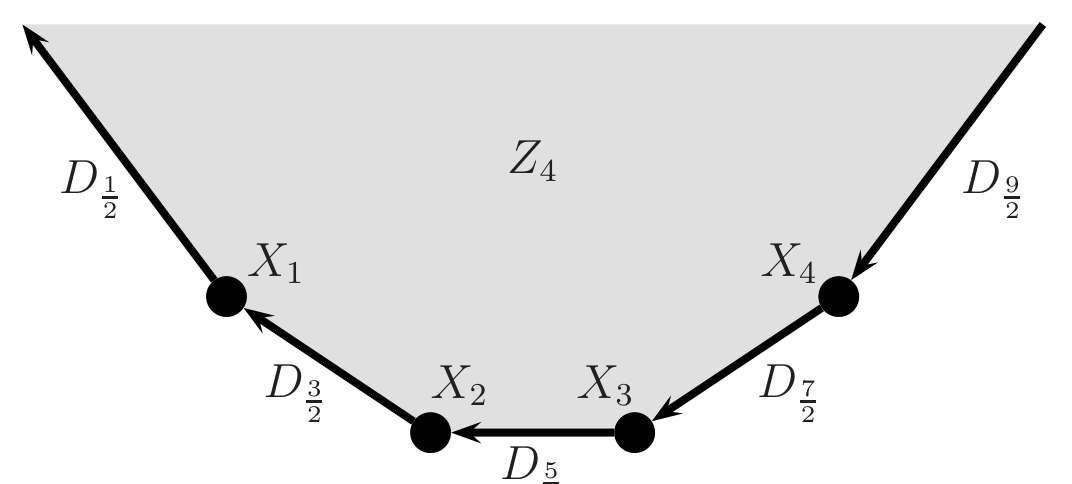
\includegraphics[width=0.56\textwidth]{figures/fig2_moment_map.png}
 \caption{纤维方向 $(\C^{\times})^2$ 作用的矩映射给出了 $Z_4$ 的示意表示。三重流形 $X_i$ 和除子 $D_s$ 分别被映到顶点和边。箭头指示 $q\to 0$ 的极限。}
  \label{f_Z4}
\end{figure}

\subsubsection{\ }
容易描述特征群之间的对偶映射
\begin{equation}
\gamma^*: H_2(Z_r,\Z) \hookrightarrow \bA^{\wedge}\,,\label{convA}
\end{equation}
格 $\bA^{\wedge}$ 由坐标特征 $\varepsilon_i$ 生成，其中 $a^{\varepsilon_i} =a_i$。它们构成与 $\{\delta_i\}$ 对偶的基。

从 $X_j$ 流向 $X_i$ 的未断裂曲线 $C_{ij}$ 的类被映到正根
$$
\gamma^*\left([C_{ij}]\right)  =  \varepsilon_i -  \varepsilon_j \,,
\quad i < j \,.
$$
而在支撑于 $\bigsqcup X_i$ 的同调类上，$\gamma^*$ 由以下公式给出。

在每个 $X_k$ 中固定一个曲线类 $\beta_k$，令
\begin{equation}
\vec \beta = \sum_k \iota_{k,*} \beta_k \in H_2(Z,\Z) \label{vecb}
\end{equation}
为它们在 $Z$ 中的并，其中 $\iota_k$ 是 $X_k$ 的包含映射。由 \eqref{DsX}，我们有
\begin{equation}
\gamma^*(\vec\beta ) = \frac{r}{2} \sum_i (L_1-L_2,\beta_i) \,
\varepsilon_i -  \frac{1}{2} \sum_{i<j} (\cK,\beta_i+\beta_j) ( \varepsilon_i -
\varepsilon_j) \,. \label{gvbe}
\end{equation}

\subsubsection{\ }
现在设 $\bigsqcup X_i$ 上的 PT 数据由如 \eqref{PTrs} 中带有截面 $s_i$ 的层集合 $\cF_i$ 指定。我们定义 $\beta_i = \ch_2 \cF_i \in H_2(X_i,\Z)$，用 \eqref{vecb} 表示这些类在 $Z$ 中的并，并令
$$
\beta = \sum \beta_i \in H_2(X,\Z)\,.
$$
由主要猜想，\eqref{PTrs} 对膜指标的贡献等于某个前因子、虚拟类贡献和相互作用 $\Phi$ 的乘积。前因子等于（包括用等变参数替换 Kähler 参数）
\begin{align}
 \textup{前因子} = & (-1)^{\chi(\cF)+\sum(r \cL_1 + (i-r)
    \cK,\beta_i)} \notag \times \\
& q^{\chi(\cF) + (\beta,\cK)/2} \, Q^{\beta} \, a^{\gamma^*(\vec\beta)}
\,.
 \label{prefC}
\end{align}
虚拟类贡献等于
\begin{equation}
  \label{vcC}
  \begin{matrix}
 \textup{虚拟类} \\
\textup{贡献}
  \end{matrix}  =
\boxtimes\,\, \Ovir \otimes \left( \Kvir \otimes \bL_{\cL_1^r \cK^{i-r}-
\cL_2^r \cK^{1-r}} \right)^{1/2} \,.
\end{equation}
最后，在相互作用项中，我们如第 \ref{s_pert} 节所述丢弃微扰项，对剩余部分得到如下等同
$$
\cX'_{ji} = N_{ji} + \overline{N_{ij}}\,,
$$
其中 $N_{ji}$ 在 \eqref{Nji} 中定义，横线表示对偶。因此，我们有
\begin{equation}
  \label{crossC}
  \textup{相互作用 $\Phi$} = \bigoplus_{i<j} \Sd
\left(\frac{a_i}{a_j} (N_{ji} +
  \overline{N_{ij}})\right)
\,.
\end{equation}
这显然开始看起来像高秩 DT 理论了，现在我们系统地检验一致性。

\subsubsection{\ }
我们从以下恒等式开始
\begin{equation}
\frac{\Sd
\left(\frac{a_i}{a_j} (N_{ji} +
  \overline{N_{ij}})\right)}
{\tSd
\left(\frac{a_i}{a_j} N_{ji} +
  \frac{a_j}{a_i} N_{ij} \right)} =
(-1)^{\rk N_{ji}}
\left(\frac{a_i}{a_j}\right)^{\!\!
- \frac12 (\rk N_{ij} + \rk
  N_{ji})}
\left(\frac{{\det N_{ij}}}{{\det N_{ji}}}\right)^{1/2}
\,. \label{SoverS}
\end{equation}
我们有
$$
\rk N_{ji} = \chi(\cF_i) - \chi(\cF_j) - (\cK,\beta_j) \,,
$$
因此特别地
$$
- \frac12 (\rk N_{ij} + \rk
  N_{ji}) = \frac12 (\cK,\beta_j+\beta_i) \,.
$$
于是由 \eqref{gvbe} 我们得出
\begin{equation}
  \label{powa}
 a^{\gamma^*(\vec \beta)} \, \left(\frac{a_i}{a_j}\right)^{\!\!
- \frac12 (\rk N_{ij} + \rk
  N_{ji})} = \prod a_i^{\frac12 r(\cL_1-\cL_2,\beta_i)}  \,.
\end{equation}
我们观察到这正是 \eqref{deftODTr} 中出现的丛 $\bL^{r/2}_{\cL_1-\cL_2}$ 的自然 $\bA$-权重。

回想我们把高秩 DT 不变量定义为在 $\bA$-不动点轨迹上的积分，因此所有线丛贡献都有一个线丛部分（在 $\bigsqcup X_i$ 的 DT 理论中定义）和一个 $\bA$-特征部分（来自把 Kähler 参数转换为等变参数）。

类似的检验发现负号与 \eqref{deftODT2r} 中前因子的符号一致。

\subsubsection{\ }
现在我们转向 \eqref{SoverS} 右端的行列式。由命题 \ref{p_symm} 和 Serre 对偶，我们有
\begin{equation}
\frac{{\det N_{ij}}}{{\det N_{ji}}} = \frac{\det \chi(\cF_j\otimes
  (\cO -\cK))}{\det \chi(\cF_i\otimes
  (\cO -\cK))} \,.\label{eq:6}
\end{equation}
因此
\begin{equation*}
\boxtimes \, \bL_{\cL_1^r \cK^{i-r}-
\cL_2^r \cK^{1-r}}
\otimes \bigotimes_{i<j} \frac{{\det
    N_{ij}}}{{\det N_{ji}}} =
\boxtimes \, \bL_{\cG_i}
\end{equation*}
其中
$$
\cG_i = \cL_1^r \cK^{i-r}-
\cL_2^r \cK^{1-r} - (2i-r-1)(\cO-\cK) \,, \quad i=1,\dots,r \,.
$$
直接计算表明
$$
\cG_i = r (\cL_1 - \cL_2) + \dots
$$
其中省略号表示 $X$ 中余维 $3$ 的 $K$-理论类，因此不影响 $\bL_{\cG}$ 形式的线丛。

这就完成了命题 \ref{p_eng} 的证明。
\section{平方根的存在性}
\label{s_sqrt}

\subsection{平方上的对称丛}

我们从以下一般观察开始。

\begin{Lemma}
设 $Y$ 是一个代数簇，$L$ 是 $Y \times Y$ 上的一个线丛，满足
$$
(12)^* L \cong L
$$
其中 $(12)$ 是因子的置换。则 $L$ 限制在对角线 $\Delta \subset Y \times Y$ 上的限制 $L_{\Delta}$ 有一个平方根。
\end{Lemma}

\noindent
我们最初的主张较弱。我们非常感激 Davesh Maulik 向我们指出这个论证在这里呈现的完全一般性下都成立。

\begin{proof}
由层的 {\'e}tale 正合列
$$
1 \to \{\pm 1\} \to \cO_Y^* \xrightarrow{f\mapsto f^2} \cO_Y^* \to 1
$$
我们得到群的正合列
$$
H^1(Y,\Z/2) \to \Pic Y \xrightarrow{\cL\mapsto \cL^{\otimes 2}} \Pic Y
\to H^2(Y,\Z/2)\,,
$$
其中最后一个映射是 $\cL \mapsto c_1(\cL)$ 模 $2$ 的约化。因此，$Y$ 上的一个线丛有平方根当且仅当它的第一 Chern 类在 $H^2(Y,\Z)$ 中可被 $2$ 整除。

由于
$$
\textup{torsion} \left(H^k(Y,\Z)\right) \cong
\textup{torsion} \left(H_{k-1}(Y,\Z)\right)
$$
群 $H^0(Y,\Z)$ 和 $H^1(Y,\Z)$ 是无挠的。因此，Künneth 分解取形式
\begin{equation}
H^2(Y \times Y,\Z) = \bigoplus_{i+j=2} H^i(Y,\Z) \otimes H^j(Y,\Z) \,.
\label{Kunn}
\end{equation}
假设 $Y$ 连通，$L$ 的对称性表明：在分解 \eqref{Kunn} 中
$$
c_1(L) = \alpha \otimes 1 +  \beta + 1 \otimes \alpha\,, \quad
\alpha \in H^2(Y,\Z),\, \beta\in \Lambda^2 H^1(Y,\Z)\,,
$$
中间部分限制到对角线上的映射是
$$
\beta_1 \otimes \beta_2 \mapsto \beta_1 \cup \beta_2
$$
由 $H^1(Y,\Z)$ 上杯积的反对称性，我们得出 $c_1(L_{\Delta})$ 是偶数。
\end{proof}

\subsection{DT 理论中的平方根}

\subsubsection{\ }

乘积上的对称线丛自然出现在三重流形的 DT 理论中。设 $\cF$ 是 $\PT(X)$ 上一维层的通用族。考虑两个 PT 模空间乘积上的线丛
$$
\bL_{12} = \det \chi(\cF_1,\cF_2)
$$

\begin{Proposition}\label{p_symm}
存在一个典范同构 $\bL_{12} \cong \bL_{21}$。
\end{Proposition}

我们期待同样的对称性对任何稳定性腔室中 $X$ 的 Donaldson-Thomas 模空间都成立。下面的证明需要修改，以考虑 $\cF$ 中的 $0$ 维子层。

注意这个陈述与 Serre 对偶的以下特例一致。假设 $\cK_X$ 平凡，令 $\bk$ 为 $\Aut X$ 作用在 $\cK_X$ 上的权重。那么 Serre 对偶给出
\begin{multline}
   \det \chi(\cF_1,\cF_2) =  \det \chi(\cF_2,\cF_1 \otimes \cK_X) =\\
=  \det \chi(\cF_2,\cF_1) \otimes \bk^{\rk \chi(\cF_2,\cF_1)} =
\det \chi(\cF_2,\cF_1) \,.
\label{deghomchi}
\end{multline}
显然，该命题由 Serre 对偶从以下推出

\begin{Lemma}\label{l_otimesL}
对 $X$ 上任意线丛 $\cL$，我们有
$$
\det \chi(\cF_1,\cF_2) = \det \chi(\cF_1,\cF_2\otimes \cL)\,,
$$
典范地。
\end{Lemma}

\begin{proof}
把 $\cL$ 写成两个极强线丛的比，我们可以约化到 $\cL$ 极强的情形。令 $s$ 为 $\cL$ 的一个一般截面。$s$ 的选择不唯一，对 $s$ 选择的依赖将在后面分析。考虑 $0$ 维层
$$
\cG = \Coker \left(\cF_2 \xrightarrow{s} \cF_2 \otimes \cL\right) \,.
$$
它有一个由 $\cO_x$（$x\in X$）的直和给出的典范滤过。对 $X$ 上任意层 $\cF$，取 $\cF$ 的局部自由分解，我们有
$$
\det \chi(\cF,\cO_x) = \left(\det \cF\right)^*_x \,,
$$
由于 $\cF_1$ 是一维的，
$$
\det \cF_1 = \cO_X
$$
这给出一个同构
$$
\phi_s: \det \chi(\cF_1,\cF_2)  \to \det \chi(\cF_1,\cF_2\otimes
\cL)\,.
$$
剩下要分析这个同构对 $s$ 的依赖。

记
$$
\Delta \subset H^0(X,\cL)
$$
为使 $\cG$ 不是 $0$ 维的截面 $s$ 的集合。这是余维 $>1$ 的锥形子集。对任意 $s_0 \in
H^0(X,\cL)\setminus \Delta$，函数 $\phi_s \phi_{s_0}^{-1}$ 关于 $s$ 是次数为
$$
\deg_s \phi_s \phi_{s_0}^{-1}  = \rk \chi(\cF_1,\cF_2) = 0
$$
的齐次函数，且在 $\Delta$ 外正则，因此恒等于 $1$。
\end{proof}

\subsubsection{\ }\label{pull_square}

我们有以下

\begin{Proposition}\label{p_Ksquare}
对任意满足 $\cL_1\otimes \cL_2 =
\cK_X$ 的 $\cL_1$ 和 $\cL_2$，我们有
$$
\Kvir \otimes \bL_{\cL_1-\cL_2} = \textup{square} \otimes
\bL_{c_1(\cL_1) \cap c_1(\cL_2)} \,,
$$
其中最后一项由 Hilbert-Chow 映射拉回。
\end{Proposition}

\begin{proof}
首先注意，对 $\cL_1=\cO_X$ 和 $\cL_2=\cK_X$，由 Serre 对偶我们有
$$
   \Kvir \otimes \bL_{\cO-\cK} = \det
\big[ \chi(\cF,\cF) - 2 \chi(\cF\otimes \cK_X)
\big] \,,
$$
由命题 \ref{p_symm}，这是一个平方。另一方面，
$$
\bL_{\cL_1-\cL_2} \otimes \bL_{\cO-\cK}^{-1} =
\bL_{\cL_1-\cO}^2  \otimes \bL_{(\cO-\cL_1)(\cO-\cL_2)} \,.
$$
写
$$
\cL_i = \cA_i \, \cB_i^{-1}\,, \quad i=1,2\,,
$$
其中 $\cA_i$ 和 $\cB_i$ 是极强的。那么
\begin{align*}
(\cO-\cL_1)(\cO-\cL_2) = \cA_1 \cA_2 \Big[
&(1-\cA_1^{-1})(1-\cA_2^{-1}) - (1-\cA_1^{-1})(1-\cB_2^{-1})\\
-&(1-\cB_1^{-1})(1-\cA_2^{-1}) + (1-\cB_1^{-1})(1-\cB_2^{-1}) \Big]
\,.
\end{align*}
由引理 \ref{l_otimesL}，右端所有项都产生丛 $\bL_{\cO_C}$，其中 $C\subset X$ 是两个极强除子的完全交。由构造，这样的丛由 Hilbert-Chow 映射拉回。显然，所得曲线的有理等价类等于 $c_1(\cL_1) \cap c_1(\cL_2)$。
\end{proof}

\subsection{M-理论中的平方根}

\subsubsection{\ }

由于稳定膜的模空间仍在构造之中，我们这里只在简化假设下做数值检验。

\begin{Proposition}
若 $\phi: B \to \MM(Z)$ 是光滑曲线到局部完全交轨迹的映射，则
$$
\deg \phi^*\Kvir \equiv \int_{\textup{$B$ 的扫过}} c_2(Z)
\mod 2 \,.
$$
\end{Proposition}

\begin{proof}
令
$$
S \subset B \times Z \times \pP^N
$$
为对应于映射 $\phi$ 的曲面，其中 $\pP^N$ 是如第 \ref{s_mapsf} 节中的辅助射影空间。由假设，$S$ 局部是完全交，因此有法丛 $N_S$。我们令
$$
N = N_{S} - T \pP^N,
$$
这是 $S$ 上一个秩 $4$ 的丛。由定义，
$$
\phi^*\Kvir = \left( \det \pi_* N \right)^{-1}
$$
其中 $\pi: S \to B$ 是投影。由 Grothendieck-Riemann-Roch，我们有
$$
\ch \pi_* N  = \pi_*  \left(\ch  N \,  \frac{\Td S}{\Td B}
\right) = \pi_*  \left(\ch  N \,  \frac{\Td Z}{\Td N}
\right) \,.
$$
由于 $\rk N = 4$，我们有
$$
\frac{ \ch N} {\Td N}  = 4 - c_1(N) + \frac{4}{3} \,
\ch_2(N)
$$
而
$$
\Td Z = 1+ \frac{1}{12} c_2(Z)
$$
因为 $c_1(Z)=0$。把所有东西放在一起，我们看到
\begin{align*}
\deg \pi_* N &= \frac{1}{3} \int_S
\left( c_2(Z) + 4 \ch_2(N) \right) \\
&\equiv  \int_S c_2(Z)  \mod 2
\end{align*}
因为 $2\ch_2$ 是整特征类，除以 $3$ 不影响奇偶性。
\end{proof}

\subsubsection{\ }

现在我们比较 DT 和 M-理论中的奇偶性计算。我们考虑
$$
Z =
\begin{matrix}
\cL_1 \oplus \cL_2  \\
\downarrow\\
X
\end{matrix} \,, \quad \cL_1 \otimes \cL_2 = \cK_X \,,
$$
是三重流形 $X$ 上秩 $2$ 丛的情形。我们有以下

\begin{Proposition}
对如上所述的 $Z$，
$$
c_2(Z) \equiv c_1(\cL_1) \, c_1(\cL_2) \mod 2 \,.
$$
\end{Proposition}

\begin{proof}
我们有
$$
c_2(Z) - c_1(\cL_1) \, c_1(\cL_2) =
c_2(X) - c_1^2(X) \equiv c_2(X) +c_1^2(X) = 12 \Td_2(X) \,,
$$
所以只需证明
$$
6 \int_D \Td_2(X) \in \Z
$$
对任意完全除子 $D\in X$ 成立。这是函数
$$
k\mapsto \dim \chi(\cO_D(kD))
$$
的整性和 Hirzebruch-Riemann-Roch 公式的一个简单推论。
\end{proof}
\section{精化不变量}\label{s_refined}

\subsection{缩放 $3$-形式的作用}

\subsubsection{\ }\label{ss_sc1}

在 M-理论构造中，最流行的流形 $Z$ 具有形式
$$
Z = X \times \C^2
$$
其中 $X$ 是 Calabi-Yau 三重流形，$\C^2\cong \R^4$ 是我们日常经验的时空（在下面所有内容中它都可以被 $A_n$ 曲面替代）。

作为这种 $Z$ 的 $\Cq$ 环面，我们可以取作用在 $\C^2$ 因子上的最大环面
$$
\begin{bmatrix}
 q \\ & q^{-1}
\end{bmatrix} \subset SL(2)
$$
由于 $\cL_1 = \cL_2 = \cO_X$，我们有
$$
\tO_{\PT} = (-q)^{\chi} \, Q^{\beta} \, \Ovir \otimes \Kvir^{1/2} \,.
$$
在本节全文中，我们将处理 DT 模空间的各个分支，并为简便起见略去前因子 $(-q)^{\chi} \, Q^{\beta}$。

\subsubsection{\ }

设 $G$ 是作用在 $X$ 上的连通群，令 $\bk$ 为这个作用的行列式，即
$$
\bk = \textup{权重}  \left(\Lambda^{3} T^{1,0} X \right)\,.
$$
字母 $\bk$ 意在让人想起典范类 $\cK_X$，只不过它是 $\cK_X$ 的 $G$-权重的\emph{逆}。

令 $\Gk$ 为 $G$ 的最小覆盖，在其上特征 $\bk^{1/2}$ 有定义。我们定义
$$
\Gk \hookrightarrow G_q = \Aut(Z,\Omega^5)^{\Cq}
$$
为
$$
 g \mapsto \left(g, \begin{bmatrix}
 \bk(g)^{-1/2} \\ & \bk(g)^{-1/2}
\end{bmatrix} \right) \,.
$$
平方根 $\bk^{1/2}$ 是使 $\cL_1 = \cL_2$ 成为 $\Gk$-等变线丛所需要的。

如果 $\bk$ 是\emph{非平凡}的，本节的结果将特别有趣。由于 $\Gk$ 在上同调上平凡作用，我们有
$$
\bk \ne 1  \Rightarrow [\Omega^3_X] = 0 \in H^3(X) \,,
$$
因此要发生这种情况，$X$ 必须是非紧的。具有 $\bk\ne 1$ 的 $X$ 的例子包括环面 Calabi-Yau 簇、局部曲线和局部曲面。

我们注意到，即使对于非紧的 $X$，PT 模空间也很可能是紧的，这在下面很重要。

\subsubsection{\ }

本节的主要结果如下

\begin{Theorem}\label{t_kappa}
对任意 Calabi-Yau 三重流形 $X$，层 $\tO_{\PT}$ 具有典范的 $\Gk$-等变结构。若 $\cM$ 是 $\PT(X)$ 的一个固有分支，则
$$
\chi(\cM,\tO_{\PT} ) \in \Z\left[\bk^{\pm 1/2}\right] \subset
K_{\Gk} (\pt) \,,
$$
即 $\Gk$ 在 $\chi(\cM,\tO_{\PT} )$ 上的作用通过特征 $\bk^{1/2}$ 分解。此外，多项式 $\chi(\cM,\tO_{\PT} )$ 关于
$$
\bk^{1/2} \mapsto \bk^{-1/2}\,.
$$
是对称的。
\end{Theorem}

对于 $\bk\ne 1$，我们猜想定理 \ref{t_kappa} 中的多项式与 \cite{BBS,BJM,KS} 及许多其他论文中研究的动机精化 DT 不变量一致。这个猜想已由 Davesh Maulik 在 \cite{Dmot} 中证明。

\subsubsection{\ }

事实上，定理 \ref{t_kappa} 的结论对任何对称完美障碍理论的层
$$
\tO_{\vir} = \Ovir \otimes \Kvir^{1/2}
$$
都成立，只要群 $\Gk$ 作用并通过一个特征 $\bk$ 缩放障碍理论的对称性
\begin{equation}
\Obs \cong \Def^{\vee} \otimes \C(\bk) \label{symm_bk}\,,
\end{equation}
其中 $\C(\bk)$ 是权重为 $\bk$ 的一维表示。

例如，在第 \ref{s_Hodge} 节中代入 $t=\bk$，我们看到
\begin{equation}
\chi \left(\Ovir \otimes \Kvir^{1/2}\right) =
\sum_{p,q} (-1)^{p-d/2} (-\bk)^{q-d/2} H^p(\Omega^q M)
\label{hpk}
\end{equation}
其中 $H^p(\Omega^q M)$ 是 $\Gk$ 的平凡表示，$d = \dim M$。
$M$ 的 Hodge 菱形的对称性
$$
h_{p,q} = h_{d-p,d-q}
$$
蕴含多项式 \eqref{hpk} 关于 $\bk^{1/2} \mapsto \bk^{-1/2}$ 的对称性。

\subsubsection{\ }

指标 \eqref{hpk} 的基本性质非常经典，可以从许多不同角度来看，特别是从 \cite{WittenMorse} 中的 Morse 理论观点来看。我们将发现 Morse 理论的观点对一般对称完美障碍理论非常有用。

$\Aut(M)_0$ 作用在 $H^p(\Omega^q M)$ 上的平凡性是\emph{刚性}的一个例子，特别参见 \cite{BT}。第 \ref{s_rig} 节中使用的论证对于读过 \cite{BT} 的人来说会非常熟悉。

\subsection{$\bk$-平凡环面的局部化}
\label{s_local}

\subsubsection{平方根上的等变结构}

在本节中，我们假设 $\cM$ 是一个射影概形，具有对称完美障碍理论以及代数群 $G$ 的作用，后者如 \eqref{symm_bk} 中那样通过特征 $\bk$ 缩放障碍理论的对称性。像以前一样，我们用 $\Gk$ 表示 $G$ 的最小覆盖，在其上特征 $\bk^{1/2}$ 有定义。

我们假设线丛 $\Kvir$ 在 $\cM$ 的非等变 Picard 群中是一个平方。由命题 \ref{p_Ksquare}，这对 PT 模空间成立。令 $\Kvir^{1/2}$ 为 $\Kvir$ 的一个平方根选择。

\begin{Proposition}\label{p_equiv12}
$\Kvir^{1/2}$ 上存在一个典范的 $\Gk$-作用。
\end{Proposition}

\begin{proof}
射影概形 $\cM$ 上的任意线丛 $\cL$ 由模
$$
\Gamma(\cL) = \bigoplus_{n\gg 0} H^0(\cL(n))
$$
在 $\cM$ 的齐次坐标环上唯一确定，而 $\cL$ 上的等变结构就是这个模上的等变结构。

逐纤维平方映射 $\Kvir^{1/2} \to \Kvir$ 给 $\Kvir^{1/2}$ 及相应的模一个典范的 $\fg$-模结构，其中
$$
\fg = \Lie G = \Lie \Gk \,.
$$
我们断言
\begin{equation}
\textup{权重} \, \Gamma(\Kvir^{1/2}(n))
\subset \textup{权重}(G) +
\Z \bk^{1/2} = \textup{权重}(\Gk) \,. \label{eq:7}
\end{equation}
事实上，令 $\bT\subset G$ 为最大环面，$\ft = \Lie
\bT$。由形变与障碍之间的对偶性，$\Kvir^{1/2}$ 在任何不动点处的 $\ft$-权重是 $\Gk$ 的一个权重。由于 $\Kvir^{1/2}(n)$ 的截面由它们在不动点处的级数展开唯一确定，\eqref{eq:7} 随之成立。

因此，$H^0(\Kvir^{1/2}(n))$ 是满足 \eqref{eq:7} 的有限维 $\fg$-模，因而积分成一个 $\Gk$-模。
\end{proof}

特别地，该命题使
$$
\tO_{\cM} = \Ovir \otimes \Kvir^{1/2}
$$
成为 $\cM$ 上的 $\Gk$-等变层。

\subsubsection{\ }

固定一个最大环面 $\bT \subset G$ 以及 $\bk$ 的核中的一个子环面 $\bA \subset \bT$。这特别意味着 $\bA$ 以典范方式作用在 $\Kvir^{1/2}$ 上。令 $\cM^{\bA}\subset \cM$ 为 $\bA$-不动点轨迹。虚拟 Euler 示性数的等变局部化取如下形式 \cite{GP,FG}。

限制到 $\bA$，障碍理论分解为
$$
\left(\Def-\Obs\right)\Big|_{\cM^{\bA}} =
\left(\Def-\Obs\right)^{\textup{fixed}} \oplus
\left(\Def-\Obs\right)^{\textup{moving}}
$$
其中运动部分是按 $\bA$ 的非平凡表示变换的部分。$\bk$ 在 $\bA$ 上的平凡性蕴含
$$
\Obs ^{\textup{fixed}} \cong \left(
\Def ^{\textup{fixed}}\right)^{\vee} \otimes \C(\bk)\,,
$$
对运动部分类似。特别地，障碍理论的不动部分定义了不动点轨迹上的一个对称完美障碍理论，带有它自己的虚拟结构层。我们有
\begin{equation}
\chi(\cM,\tO_{\cM}) = \chi\left(\cM^{\bA}, \cO_{\cM^{\bA},\textup{vir}}
\otimes \Kvir^{1/2}\big|_{\cM^{\bA}} \otimes \Sd \cN^{\vee} \right)\,,
\label{vir_loc}
\end{equation}
其中
$$
\cN = \left(\Def-\Obs\right) ^{\textup{moving}}
$$
是虚拟法丛。

我们的下一个目标是使用对不动点轨迹的虚拟典范丛的一个特定平方根选择来重写公式 \eqref{vir_loc}。

\subsubsection{\ }

出现在 $\cN$ 中的 $\bA$-权重把 $\Lie \bA$ 划分为有限多个腔室。我们固定一个腔室 $\fC$，它把所有权重分为正和负，因此我们可以写
$$
\cN =
\cN_{+} \oplus
\cN_{-}
$$
其中
$$
\cN_{-} = - \cN_{+}^{\vee}
\otimes \C(\bk) \,.
$$
我们有以下

\begin{Lemma}
非等变线丛 $\det \cN_+$ 不依赖于 $\fC$ 的选择，且满足
$$
\det \cN = (\det \cN_+)^2 \,.
$$
\end{Lemma}

\begin{proof}
令 $\fC_1$ 和 $\fC_2$ 是两个腔室，用 $\cN_{\pm,\pm}$ 表示由在 $\fC_1$ 和 $\fC_2$ 上具有给定符号的特征所张成的 $\cN$ 的部分。那么
$$
\cN_{+,-} = - \cN_{-,+}^{\vee}
$$
由此
$$
\det \cN_{+,-} = \det \cN_{-,+}
$$
这蕴含独立性。特别地 $\det \cN_+ =
\det \cN_-$，因此
$$
\det \cN = \det \cN_+  \det \cN_- = (\det \cN_+)^2 \,.
$$
\end{proof}

我们利用命题 \ref{p_equiv12} 的证明所提供的典范 $\bT_{\bk}$-等变结构赋予 $\det \cN_+$，并令
\begin{equation}
\cK_{\cM^{\bA}}^{1/2} = \det \cN_+
\otimes \Kvir^{1/2} \big|_{\cM^{\bA}} \label{eq:9}
\end{equation}
这为不动点轨迹提供了一个一致的平方根选择，它依赖于 $\cM$ 上平方根的选择。

\subsubsection{\ }

我们记
$$
\tO_{\cM^{\bA}} = \cO_{\cM^{\bA},\textup{vir}} \otimes
\cK_{\cM^{\bA}}^{1/2}
$$
并令 $\rho$ 为从等变 $K$-理论到其完备化的映射，使得
$$
\rho(A\oplus B) = \rho(A) \otimes \rho(B)
$$
且对线丛 $\cL$
$$
\rho(\cL) = \frac{\bk^{1/2}-\bk^{-1/2} \cL}{\cL-1}
$$
利用 \eqref{eq:9} 和对偶性重写 \eqref{vir_loc}，我们得到以下

\begin{Proposition}\label{p_rho}
对任意腔室 $\fC\subset \Lie \bA$，我们有
\begin{equation}
\chi(\cM,\tO_{\cM}) = \chi\left(\cM^{\bA}, \tO_{\cM^{\bA}}
\otimes \rho(\cN_{+}) \right) \,.
\label{vir_loc2}
\end{equation}
\end{Proposition}

\subsection{Morse 理论与刚性}

\subsubsection{不动分支的虚拟指标}

我们记
\begin{align}
  \sind_{\fC} &=
\rk \cN_+\notag \\
&= \rk \Def_+ - \rk \Def_- \label{sind} \,,
\end{align}
其中两行之间的相等性来自 $\Obs_+$ 与 $\Def_-$ 之间的对偶性；这也表明第二行不依赖于障碍理论的特定代表。

显然，$\sind_{\fC}$ 是 $\cM^{\bA}$ 上的局部常值函数，我们称之为不动分支的虚拟指标。

\subsubsection{刚性}\label{s_rig}

\begin{Proposition}\label{p_rig}
$\Gk$ 在 $\chi(\cM,\tO_{\cM})$ 上的作用通过特征 $\bk^{1/2}$ 分解。事实上，
\begin{equation}
  \label{eq:11}
  \chi(\cM,\tO_{\cM}) = \chi\left(\cM^{\bA}, \tO_{\cM^{\bA}}  \otimes
    (-\bk^{1/2})^{\sind_{\fC}} \right)
\end{equation}
对 $\bA = \bT \cap \Ker \bk$ 的 Lie 代数中的任意腔室 $\fC$ 成立，其中 $\bT$ 是 $G$ 的最大环面。
\end{Proposition}
\begin{proof}
只需证明 $\bT_{\bk}$ 在 $\chi(\cM,\tO_{\cM})$ 上的作用通过特征 $\bk^{1/2}$ 分解。由于 $\cM$ 是紧的，$\chi(\cM,\tO_{\cM})$ 的 $\bT_{\bk}$-特征是一个 Laurent 多项式，我们断言它在 $\bA$-陪集上是常值。

令 $\sigma: \C^{\times} \to \bA$ 为一个一般的同态，令 $\fC$ 为包含 $d\sigma \in \Lie\bA$ 的腔室。那么出现在 $\cN_+$ 中的所有特征在 $\sigma(z)$ 上当 $z\to 0$ 时趋于零，当 $z\to\infty$ 时趋于无穷。因此，对任意 $t\in\bT$ 我们有
\begin{alignat*}{2}
   \chi(\cM,\tO_{\cM})\big|_{t \sigma(z)}
 &= \chi\left(\cM^{\bA}, \tO_{\cM^{\bA}}  \otimes
    (-\bk^{1/2})^{\sind_{\fC}} \right)  + O(z)\,, \quad &&z\to 0 \\
&= \chi\left(\cM^{\bA}, \tO_{\cM^{\bA}}  \otimes
    (-\bk^{1/2})^{-\sind_{\fC}} \right)  + O(z^{-1})\,, \quad &&z\to \infty
  \,.
\end{alignat*}
由于这是 $z$ 的 Laurent 多项式，它是一个常数，等于它在 $0$ 或 $\infty$ 处的值。由于 $\sigma$ 是一般的，断言随之成立。
\end{proof}

\subsubsection{定理 \ref{t_kappa} 证明的结论}

剩下要证明 $\bk\mapsto\bk^{-1}$ 的对称性。由于任何自对偶理论的虚拟维数为 $0$，由 \cite{FG} 的弱 Serre 对偶定理我们得到
$$
\chi(\tO_{\cM}) = \chi(\tO_{\cM})^{\vee}
$$
且由于 $\bk^{\vee} = \bk^{-1}$，我们就完成了证明。
\section{指标顶点与精化顶点} \label{s_index_vertex}

\subsection{环面 Calabi-Yau 三重流形}

\subsubsection{\ }

在本节中，我们把第 \ref{s_refined} 节的讨论特殊化到环面 Calabi-Yau 三重流形 $X$。对于这样的 $X$，环面
$$
\bA = \bT \cap \Ker \bk \cong \left(\C^{\times}\right)^2
$$
在曲线的 Hilbert 概形上以孤立不动点作用，因此 $X$ 的 K-理论 DT 不变量可以由一个与 $X$ 的同调 DT 不变量的局部化公式 \cite{mnop} 具有相同风格的组合公式给出，后者在拓扑顶点 \cite{AKMV,ORV} 的形式体系中为许多人所熟知。

\subsubsection{\ }

令
$$
\Delta(X) \subset \left(\Lie \bT\right)^*
$$
为环面多面体，即 $X$ 上某个 Kähler 类的矩映射的像。它的 $1$-骨架在 $\left(\Lie \bA\right)^*$ 上的投影称为 $X$ 的环面图。这些对象的组合类型不依赖于 Kähler 类的选择。

\begin{figure}[!htbp]
  \centering
   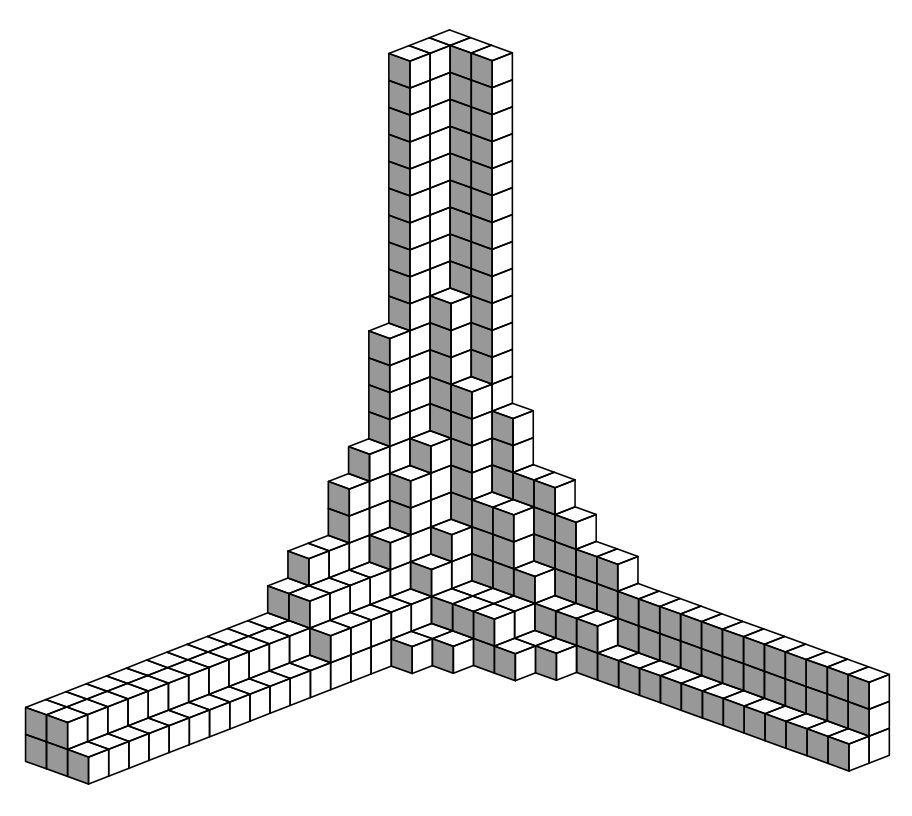
\includegraphics[width=0.42\textwidth]{figures/fig3_partition_legs.png}
 \caption{一个三腿的三维分拆}
  \label{f_part}
\end{figure}

所谓带腿的三维分拆，我们指的是图 \ref{f_part} 所示类型的对象。它们与 $\cO_{\C^3}$ 中 $\bA$-固定的一维理想一一对应。一般环面 $X$ 上的 $\bA$-固定理想层由放置在 $\Delta(X)$ 顶点上的三维分拆集合 $\{\pi_v\}$ 描述，这些分拆沿 $\Delta(X)$ 的边粘合。此外，沿 $\Delta(X)$ 的无界边不允许有非平凡的腿。这些规则如图 \ref{f_Om1Om1} 所示。

\subsubsection{\ }

$\PT(X)^{\bA}$ 的描述非常相似，见 \cite{PT2}。我们这里讨论 Hilbert 概形上的局部化，因为我们想与 Iqbal、Kozcaz 和 Vafa 的精化顶点 \cite{IKV} 建立联系。

由于 $\Hilb(X)$ 从不紧，命题 \ref{p_rig} 不能直接应用于它。然而，如果 $\PT(X)$ 是紧的，并且我们假设推测公式 \eqref{ePTDT}，那么精化不变量对腔室的唯一依赖来自 $X$ 的点 Hilbert 概形。

我们有
$$
\chi\left(X, \cK_X^{1/2} \otimes
(TX + \cK_X - T^*X- \cK_X^*)\right) = \sum_{x\in X^{\bT}}
\rho(T_x X)
$$
因此由猜想 \ref{c_DT0} 我们有
\begin{multline}
\lim_{z\to 0} \,
\chi\left(\Hilb(X,\textup{points}),\tO_{\textup{vir}}\right) \Big|_{t\sigma(z)}= \\
\Sd \frac{q}{(1-q\bk^{1/2})(1-q\bk^{-1/2})}
\sum_{x\in X^T} \left(-\bk^{1/2}\right)^{\sind_{\sigma}(x)}\label{atoinf} \,,
\end{multline}
对任意同态 $\sigma: \Ct \to \bA$，其中
$$
\sind_{\sigma}(x) = \dim (T_x X)_+- \dim (T_x X)_-  = \pm 1
$$
是 $x\in X^T$ 关于 $\sigma$ 的指标。\eqref{atoinf} 中对 $x$ 的求和是 $X$ 的 Poincaré 多项式的等变类似物；它在 $\Lie A$ 中与环面图的无界边对偶的壁上跳跃。

\begin{figure}[!htbp]
  \centering
   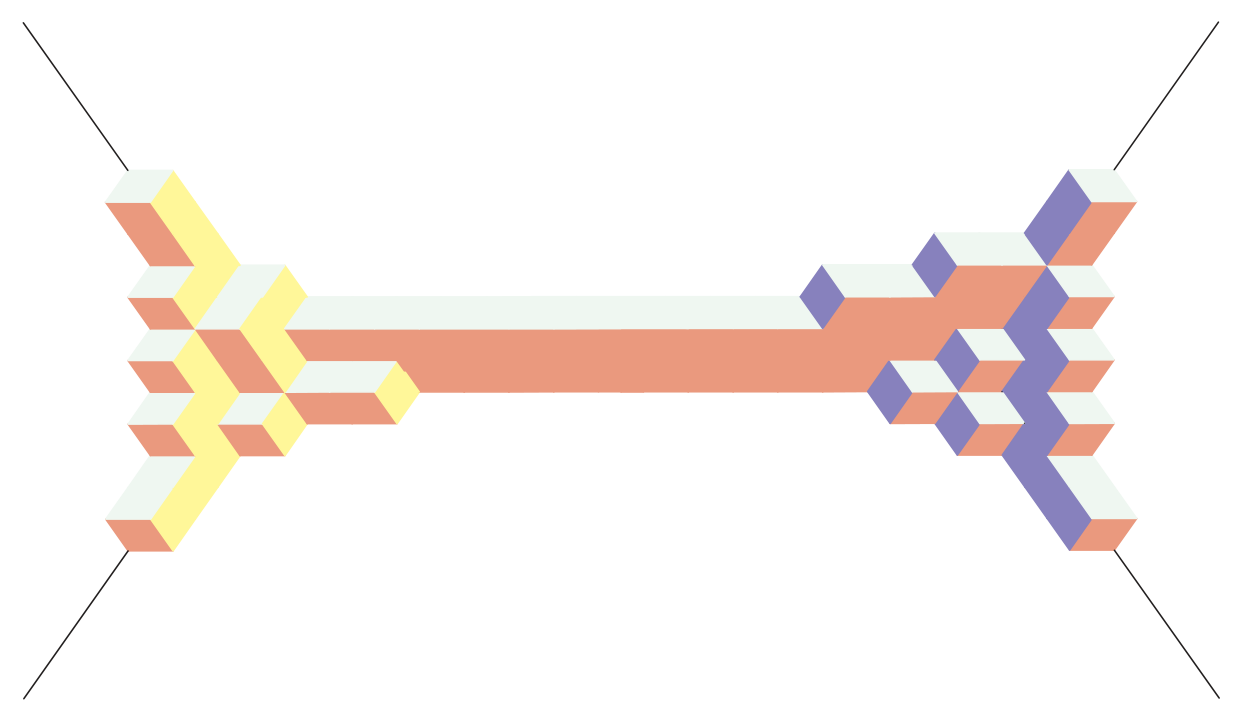
\includegraphics[width=0.56\textwidth]{figures/fig4_ideal_sheaf.png}
 \caption{$\cO(-1)\oplus\cO(-1)\to \pP^1$ 上的一个 $\bA$-固定理想层}
  \label{f_Om1Om1}
\end{figure}

\subsection{不动点处的虚拟切空间}

\subsubsection{\ }

对三重流形 $X$ 上一个 $\bT$-固定的理想层 $\cI$，我们记
$$
\cN(\cI) = \chi(\cO_X) -
  \chi(\cI,\cI) \,.
$$
对 $\cI\in \Hilb(X)^{\bT}$，这是 $\cI$ 处的虚拟切（和虚拟法）空间。对一维单项式理想
$$
I \subset \C[x_1,x_2,x_3] = \cO_{\C^3}
$$
$\cN(I)$ 的特征作为
$$
\cN(I) \in \Q(\bT) \supset K_{\bT}(\pt) \,.
$$
的元素是良定义的。事实上，$\tr_{\cN(I)}$ 仅有的极点是在无穷腿方向的权重 $t_i$ 处的一阶极点，见 \cite{mnop}。对任意 $\cI$ 我们有
$$
\cN(\cI) = \sum_{x \in X^{\bT}}  \cN(I_x) \,,
$$
其中 $I_x$ 是 $\cI$ 在 $x$ 处环面坐标卡上的限制，见 \cite{mnop}。

\subsubsection{\ }

$\tr_{\cN(I)}$ 在 $t_1=1$ 处的留数只依赖于 $I$ 关于 $x_1$ 的饱和化
$$
I^{\textup{leg}}_1 \supset I
$$
组合上，$I^{\textup{leg}}_1$ 对应于 $x_1$ 方向上一条纯无穷腿，其与 $I$ 有相同的截面 $\lambda$。我们有
$$
\cN(I^{\textup{leg}}_1) = \C[x_1] \otimes
T_{I_{\lambda}} \Hilb(\C^2)\,,
$$
其中 $I_{\lambda} \subset \C[x_2,x_3]$ 是相应的单项式理想。

如果 $e$ 是 $\Delta(X)$ 中连接两个顶点 $x$ 和 $x'$ 的一条边，则相应的饱和化 $I^e_{x}$ 和 $I^e_{x'}$ 粘合成一个理想层 $\cI^e$。它的形变和障碍可以用公式
$$
\cN(\cI^e) = \cN(I^e_{x}) + \cN(I^e_{x'})
$$
以及用 $\lambda$ 的方格的臂和腿对 $T_{I_{\lambda}} \Hilb(\C^2)$ 的显式描述来容易理解。

\subsubsection{\ }

我们令
$$
\cNr(I)=\cN(I) - \sum_{i=1}^3 \cN(I^{\textup{leg}}_i) \in K_{\bT}(\pt) \,.
$$
它满足
$$
\cNr(I) = - \C(\bk) \otimes \cNr(I)^{\vee} \,.
$$
由构造，
$$
\cN(\cI) = \sum_{\textup{边 $e$}} \cN(\cI^e) +
\sum_{\textup{顶点 $x$}}  \cNr(I_x) \,.
$$
由于第一项是显式的，我们聚焦于顶点贡献。

\subsubsection{K-理论顶点}\label{s_K_vertex}

由命题 \ref{p_rho} 我们得到局部化顶点的如下公式
\begin{equation}
\bV(\lambda,\mu,\nu) = \sum_{\pi} (-q)^{|\pi|} \,
\rho\left(\cNr(I)_+\right)\,,
\label{full_vert}
\end{equation}
其中求和遍历以给定的二维分拆三元组 $(\lambda,\mu,\nu)$ 为端点的所有三腿分拆 $\pi$，$I\in \cO_{\C^3}$ 是相应的理想，无穷分拆 $\pi$ 的大小定义为一个有限维虚 $\bT$-模的秩
$$
|\pi| = \rk \left(-2\cO-I+\sum I^{\textup{leg}}_i\right)
$$
注意这个大小可以是负的。分解
$$
\cNr(I) = \cNr(I)_+ - \C(\bk) \otimes \cNr(I)^{\vee}_{+}
$$
是关于 $d\sigma\in \Lie \bA$ 上权重的符号的，其中 $\sigma: \Ct \to \bA$ 是一般的 $1$-参数子群。乘积 $\rho\left(\cNr(I)_+\right)$ 不依赖于 $\sigma$ 的选择。

\subsubsection{指标顶点}

现在我们计算 \eqref{full_vert} 在 $t\sigma(z)\in \bT$ 上当 $z\to 0$ 时的极限。这确实依赖于 $\sigma$ 的选择，由于 $\bA$ 是二维的，我们称其为\emph{斜率}的选择。因为我们希望斜率是一般的，我们这样选取使得
\begin{equation}
\Q_{>0} \cdot d\sigma  =
\Q_{>0} \cdot \left(d\sigma_0 + \textup{小扰动}\right)\label{ray_sigma}
\end{equation}
对某个固定的有理斜率 $d\sigma_0$ 和给定符号的无穷小扰动。给定这样的一般斜率，我们定义
\begin{align}
  \label{index_vert}
  \bV^{\sigma}(\lambda,\mu,\nu) &= \lim_{z\to 0} \,
\bV(\lambda,\mu,\nu)\big|_{t \sigma(z)} \\
&=
\sum_{\pi} (-q)^{|\pi|} \,
(-\bk^{1/2})^{\sind_{\sigma} I} \,, \notag
\end{align}
其中
\begin{equation}
\sind_{\sigma} I = \rk \cNr(I)_+ \,. \label{slope_index}
\end{equation}
当 \eqref{ray_sigma} 中小扰动的符号改变时，即当射线 $\Q_{>0} \cdot d\sigma$ 从 $\Q_{>0} \cdot d\sigma_0$ 的一侧跨到另一侧时，这个值跳跃。这种壁穿越在 \cite{AO} 中分析。

\subsection{精化顶点}

\subsubsection{\ }

若 $\sigma_0$ 固定坐标轴之一，我们称斜率 $\sigma$ 是\emph{首选的}。按照约定，我们选取 $x_3$-轴，我们把它画成竖直的。在本节中，我们证明对于首选斜率，指标顶点退化为 \cite{IKV} 的精化顶点。

对于一般斜率，指标 \eqref{slope_index} 是三维分拆的一个相当复杂的函数，因为 $\cNr(I)$ 的特征对 $I$ 本身的特征是二次依赖。然而，对于首选斜率，$\rk \cNr(I)_+$ 中有大量的抵消，依赖变成线性的，即指标可以通过对 $\pi$ 中方块 $\bx\in\pi$ 的某个单和来计算。

\subsubsection{\ }

设 $\pi$ 是三维分拆，$\pi^{\textup{leg}}_3$ 是它在首选方向上的腿，$\lambda$ 是相应的二维分拆。我们把图看作平面中 $\lambda \subset \R_{\ge 0}^2$ 的方格集合，并记
$$
f_{\lambda} = \textup{boundary} \left(\R_{\ge 0}^2 \setminus \lambda
\right)
$$
为 $\lambda$ 的\emph{轮廓}。这是一条从 $x_1$-轴到 $x_2$-轴的锯齿形线。我们用相应的变量 $x_i$ 标记它的两种可能斜率，并称它的角为峰和谷，使得
\begin{equation*}
  f_{\varnothing} = \{x_1\ge 0, x_2=0\} \cup \{x_1= 0, x_2\ge 0\}
\end{equation*}
有一个谷而没有峰。更形式化的定义见下面的 \eqref{profile}。

\subsubsection{\ }

存在一个自然的投影
$$
p: \R^3 \to f_{\lambda}
$$
沿 $(1,1,0)$ 和 $(0,0,1)$ 方向。对方块 $\bx\in\pi$，我们定义
$$
\xi_{\lambda}(\bx) =
\begin{cases}
x_1\,, & p(\bx) \in \textup{$f_{\lambda}$ 的 $x_1$-斜率段}\,,\\
x_2\,, & p(\bx) \in \textup{$f_{\lambda}$ 的 $x_2$-斜率段}\,, \\
x_3^{\pm 1}\,, & p(\bx) \in \textup{$f_{\lambda}$ 的峰/谷} \,.
\end{cases}
$$
如图 \ref{f_chim} 所示。我们定义
\begin{equation}
\Xi(\pi) = \sum_{\bx \in \pi\setminus \pi^{\textup{leg}}_3}
\xi_{\lambda}(\bx) -
\sum_{\bx \in \pi^{\textup{leg}}_1}
\xi_{\varnothing}(\bx)
-
\sum_{\bx \in \pi^{\textup{leg}}_2}
\xi_{\varnothing}(\bx)\,, \label{Xip}
\end{equation}
这是一个有限和。

对首选斜率，指标由以下计算

\begin{Theorem}\label{t_pref}
若 $x_3$ 被 $\sigma_0$ 固定，则
$$
\sind_{\sigma} I = \rk \left(\Xi - \Xi^{\vee}\right)_{+} \,.
$$
\end{Theorem}

\noindent
当然，应该始终记住单项式 $x_i$ 的 $\bT$-权重是坐标方向权重的\emph{相反数}。

\subsubsection{\ }

定理 \ref{t_pref} 的证明将分几步。第一步是约化到情形
\begin{equation}
\pi^{\textup{leg}}_1=\pi^{\textup{leg}}_2=\varnothing  \,.
\label{trunc12}
\end{equation}
引入如下截断
$$
I_N = I + (x_1^N,x_2^N) \,,
$$
以及饱和化 $I^{\textup{leg}}_i$ 的相应截断 $I^{\textup{leg}}_{i,N}$。定理 \ref{t_pref} 的一般情形由以下约化到 \eqref{trunc12}

\begin{Lemma} 我们有
$$
\sind_{\sigma} =\rk\left( \cNr(I_N) - \cNr(I^{\textup{leg}}_{1,N}) -
 \cNr(I^{\textup{leg}}_{2,N})\right)_{+}
$$
对所有 $N\gg 0$ 成立。
\end{Lemma}

\begin{proof}
用 $Z$ 表示 $\cO/I$ 的谱，使得
$$
\cO_{Z_N} = \cO_Z-x_1^N \cO_{Z^{\textup{leg}}_1} -
x_2^N \cO_{Z^{\textup{leg}}_2} \,.
$$
我们计算
\begin{multline}
 \cNr(I) - \cNr(I_N) + \cNr(I^{\textup{leg}}_{1,N}) +
 \cNr(I^{\textup{leg}}_{2,N})  = \\
-\chi\left(\cO_{Z_N\setminus Z^{\textup{leg}}_{1,N}},
x_1^N \cO_{Z^{\textup{leg}}_{1}}\right) -
\chi\left(\cO_{Z_N\setminus Z^{\textup{leg}}_{2,N}},
x_2^N \cO_{Z^{\textup{leg}}_{2}}\right) \label{expandN} \\ -
\chi\left(x_1^N \cO_{Z^{\textup{leg}}_{1}},
x_2^N \cO_{Z^{\textup{leg}}_{2}}\right) - \dots
\end{multline}
其中省略号表示通过交换 Euler 示性数中两项的顺序得到的另外三个项。由于 \eqref{expandN} 中所有对的支集沿不同坐标轴延伸，每个 Euler 示性数都是 $K_{\bT}(\pt)$ 中的零维元素，被 $\sigma_0$ 的一个很大的非平凡权重平移。因此它对指标没有贡献。
\end{proof}

\subsubsection{平衡引理}\label{s_bal}

可以更抽象地思考情形 \eqref{trunc12}。设 $C$ 是某个一般三重流形 $X$ 的 $X^{\sigma_0}$ 的一维分支，手头的情形是 $X=\C^3$ 中的 $x_3$-轴。设 $Z$ 是包含在 $C$ 的无穷小邻域中的 $\bA$-不变子概形，令 $E \subset Z$ 为 $Z$ 的一般点沿 $C$ 的闭包，例如在我们的具体情形中
$$
E = Z^{\textup{leg}}_3
$$
我们定义
\begin{equation}
\Xi_Z = \chi\!\left(\cI_E,\cO_{Z\setminus E}
\otimes \left(\pi^* TC\right)^{\otimes{N}}\right)\,,\label{XiZ}
\end{equation}
其中 $TC$ 是 $C$ 的切丛，$\pi: Z \to C$ 是 $\bT$-等变投影，且
$$
0 \ll N \ll \| \textup{小扰动} \|^{-1}
$$
这里的小扰动指的是 \eqref{ray_sigma}。

以下技术结果把 $Z$ 的形变与 $E$ 的形变比较，表明差的指标关于 $[\cO_{Z}]$ 是线性的。

\begin{Lemma}\label{l_bal} 我们有
  \begin{equation}
    \label{bal}
\rk \left(\cN(Z) - \cN(E)\right)_+ = \rk \left(\Xi_Z - \Xi_Z^{\vee}\right)_+ \,.
  \end{equation}
\end{Lemma}

\noindent
这个引理的证明在附录中给出。显然，该引理在检验定义 \eqref{XiZ} 退化为公式 \eqref{Xip} 后就证明了定理。

\subsubsection{证明的结论}\label{s_chim}

现在我们回到情形 $X=\C^3$，$C$ 是 $x_3$-轴，$I_E=I^{\textup{leg}}_3$ 由 $x_1$ 和 $x_2$ 的单项式生成。具体地，
$$
I_E = \left(\left\{x_1^i x_2^j\right\}_{(i,j)\notin \lambda}\right)
$$
其中 $\lambda\in \Z_{\ge 0} \times \Z_{\ge 0}$ 是分拆的图。例如，情形
$$
I_E = (x_1^2,x_2^3)
$$
如图 \ref{f_chim} 所示。直观上，可以把 $E$ 比作房间角落里的烟囱，而 $Z$ 对应于靠在这个烟囱上堆放的几个盒子（违反所有建筑规范），如图 \ref{f_chim}。

\begin{figure}[!htbp]
  \centering
   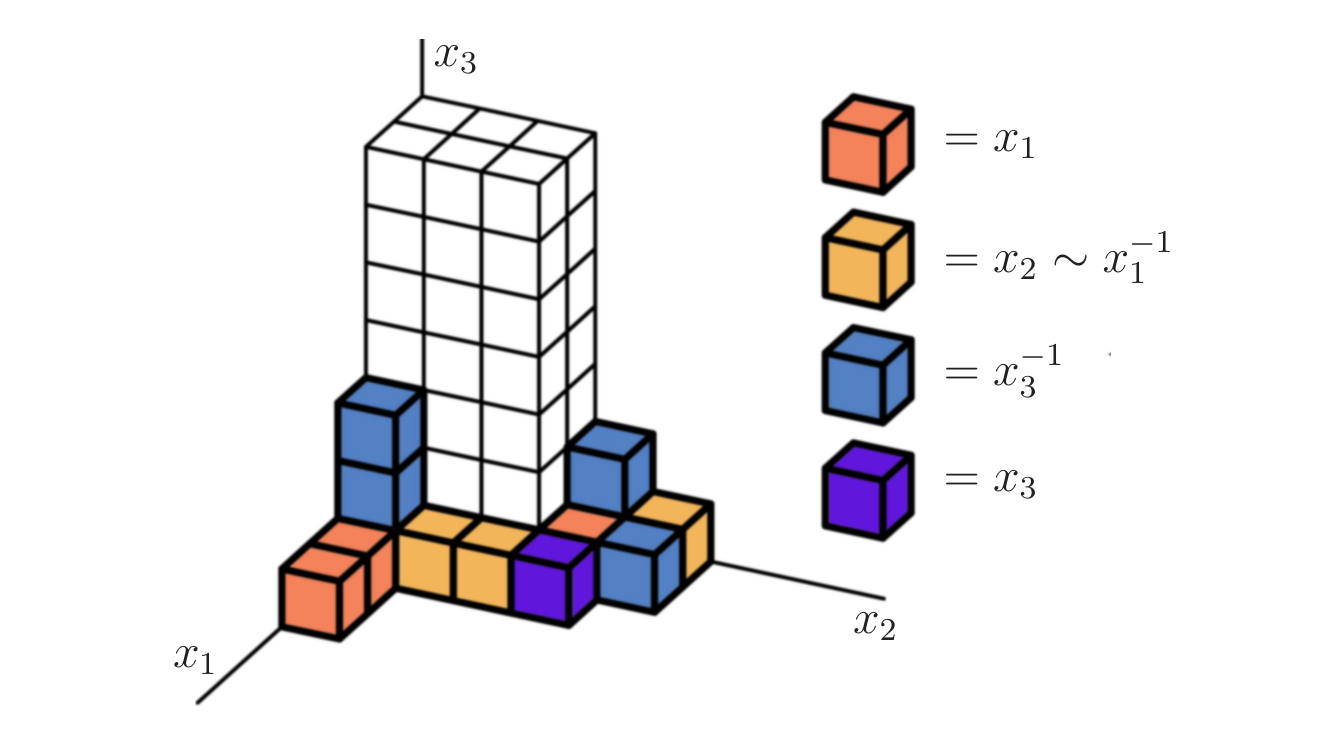
\includegraphics[width=0.72\textwidth]{figures/fig5_chimney.png}
 \caption{函数 $\xi_{\lambda}(\bx)$}
  \label{f_chim}
\end{figure}

理想 $I_E$ 的生成元和关系对应于烟囱的内角和外角，即 $\lambda$ 轮廓的谷和峰。在我们的例子中，我们有次数为 $x_1^2$ 和 $x_2^3$ 的生成元，以及一个次数为 $x_1^2 x_2^3$ 的关系。一般地，我们用
$$
\gamma_i,\rho_i \in \Z_{\ge 0}^2  \subset \Z^3
$$
表示 $I_E$ 的生成元和关系的多指标次数。于是我们有一个等变自由分解
\begin{equation}
0 \to \bigoplus_{i=1}^{g-1}  x^{\rho_i}  \cO_{\C^3}
\to \bigoplus_{i=1}^g  x^{\gamma_i}  \cO_{\C^3} \to
I_E \to 0
\label{free_res}
\end{equation}
其中 $g$ 是生成元的个数（内角的个数）。

由于 $x_3\in T^*C$ 的 $\bA$-权重是 $TC$ 权重的负，单项式 $x^{\bx}\in \cO_{Z\setminus E}$ 对 $\Xi_Z$ 指标的贡献等于以下 $\bA$-模块的 $\sigma$-指标
$$
\Xi_{\bx}= x_3^{-N} \sum_{i=1}^g{x^{\bx-\gamma_i}} + x_3^{N}
\sum_{i=1}^{g-1}{x^{\rho_i-\bx}} \,.
$$
这个指标计算如下。我们可以假设
$$
d\sigma  =  x_1 \frac{\partial}{\partial x_1}
- x_2 \frac{\partial}{\partial x_2} \,.
$$
考虑函数
$$
c((a_1,a_2,a_3)) = a_1 - a_2 \,.
$$
显然，$d\sigma_0 \cdot x^{\bx} = c(\bx)\, x^{\bx}$。$c(\bx)$ 的水平集是图 \ref{f_chim} 中的对角切片。令 $f_{\lambda}(s)$ 为 $\lambda$ 的轮廓，定义为
\begin{equation}
\tfrac{1}{2} f''_{\lambda} = \sum \delta_{c(\gamma_i)}
- \sum \delta_{c(\rho_i)}\,,\label{profile}
\end{equation}
连同
$$
f_{\lambda}(s) = |s|\,, \quad |s| \gg 0 \,.
$$
那么
$$
\sind_{\sigma} \Xi_{\bx} = f'_{\lambda}(c(\bx))
$$
根据 $x_3$ 的权重由左连续或右连续延拓。这在图 \ref{f_chim} 中用颜色编码。显然，
$$
\sind_{\sigma} \Xi_{\bx} = \xi_{\lambda}(\bx)
$$
这就完成了证明。

\appendix

\section{附录}

\subsection{平衡引理的证明}

\subsubsection{\ }

由于 $\cO_{Z}/\cO_{E}$ 是零维的，引理 \ref{l_bal} 的陈述是纯局部的，我们可以假设处于第 \ref{s_chim} 节的情境中。

我们从特殊情形 $E=\varnothing$ 开始，此时 $\cN(E)=0$。我们需要证明
\begin{equation}
\cN(Z) \equiv x_3^{-N} \, \chi(\cO_Z) -
x_3^{N} \, \overline{\chi(\cO_Z)}
\label{bal1}
\end{equation}
对所有充分大的 $N$ 成立，其中 $\bA$-模上的关系 $\equiv$ 表示它们有相同的 $\sigma$-指标。

\subsubsection{\ }

事实上，只需取 $N$ 使得 $x_3^N \in \cI_Z$，换句话说，$N$ 大于对应于 $Z$ 的盒子堆的高度。正如我们将看到的，\eqref{bal1} 左右两端之间的差对应于
$$
\cF = \pi_{12*} \left(\cI_{Z}/x_3^N \right)\,.
$$
的形变。这里 $\pi_{12}$ 是到 $(x_1,x_2)$-平面的投影，$\pi_{12*}$ 表示我们把 $\cI_{Z}/x_3^N$ 看作 $\cO_{\C^2}=\C[x_1,x_2]$-模，即 $\C^2$ 上一个（退化的）带框架秩 $N$ 瞬子。

在 $\C^2$ 原点之外，$\cF$ 与
$$
\cF_{\varnothing} = \sum_{i=0}^{N-1} x_3^i \, \cO_{\C^2}\,.
$$
相同。因此 $\bA$ 在 $x_3$ 上的作用转化为 $\cF$ 框架上的作用。

\subsubsection{\ }

$\C^2$ 上带框架的无挠层的模空间是一个光滑流形，切空间为
\begin{equation}
\cN_2(Z) = \chi_{\C^2}(\cF_{\varnothing},\cO_Z)
+  \chi_{\C^2}(\cO_Z,\cF_{\varnothing}) - \chi_{\C^2}(\cO_Z,\cO_Z) \,,
\label{Xi2F}
\end{equation}
其中 $\chi_{\C^2}$ 表示我们把所有层视为 $\bA$-等变 $\cO_{\C^2}$-模。特别地，
$$
\chi_{\C^2}(\cO_0,\cO_0) = (1 - x_1^{-1}) (1- x_2^{-1}) =
(1-x_3^{-1})^{-1}\, \chi(\cO_0,\cO_0)
$$
其中 $0\in \C^2\subset \C^3$ 是原点。由此得出
$$
\cN(Z) = (1-x_3^{-1}) \, \cN_2(Z) + x_3^{-N} \, \chi(\cO_Z) -
x_3^{N} \, \overline{\chi(\cO_Z)}
$$
因此，\eqref{bal1} 等价于证明
\begin{equation}
\sind_{\sigma} \, \cN_2(Z) = 0
\label{bal2}
\end{equation}

\subsubsection{\ }

$\C^2$ 上的辛形式 $dx_1 \wedge dx_2$ 在瞬子模空间上诱导一个辛形式，特别地在 $\cF$ 的切空间 $\cN_2(\cF)$ 上诱导辛形式 $\omega_{\cF}$。环面 $\bA$ 以 $x_1 x_2$ 的权重缩放这个辛形式，这与 $x_3^{-1}$ 的权重相同。因此，$\omega_{\cF}$ 把吸引和排斥方向配对，除了权重 $0$ 和 $x_3^{-1}$。因此 \eqref{bal2} 由以下推出

\begin{Lemma}
$$
\cN_2(Z)^{\bA} = 0\,.
$$
\end{Lemma}

\begin{proof}
我们有
$$
\cF = \bigoplus_{i=1}^N x_3^{i-1} \, \cI_{\lambda^{(i)}}
$$
其中 $\cI_{\lambda} \subset \C[x_1,x_2]$ 是对应于分拆 $\lambda$ 的单项式理想，且
$$
\lambda^{(1)} \supset \lambda^{(2)} \supset \dots \supset
\lambda^{(N)} \,.
$$
因此
$$
\cN_2(Z) = \sum_{i,j}
x_3^{j-i}\left(\chi_{\C^2}(\cO_{\C^2}) -
\chi_{\C^2}
\left(\cI_{\lambda^{(i)}},\cI_{\lambda^{(j)}}\right)
\right)
$$
于是断言由以下引理 \ref{l_incl} 得出。
\end{proof}

\subsubsection{\ }

\begin{Lemma}\label{l_incl}
设 $\cI,\cJ\in \C[x_1,x_2]$ 是单项式理想。若
$$
(n <0 \textup{ 且 } \cI \supset \cJ) \textup{ 或 }
(n \ge 0 \textup{ 且 } \cI \subset \cJ)
$$
则权重 $(x_1 x_2)^n$ 不出现在
$$
\chi_{\C^2}(\cO_{\C^2}) -
\chi_{\C^2}
\left(\cI,\cJ\right)\,.
$$
\end{Lemma}

\begin{proof}
由对偶性，只需考虑情形 $\cI \supset \cJ$。由类似 \eqref{free_res} 的分解，我们有
\begin{equation}
  \supp \, \chi_{\C^2}
\left(\cI,\cJ\right)
\subset
  \bigcup_{i,j}
\supp \,\, x^{b_j-a_i} \cO_{\C^2} \,,
\label{suppsupp}
\end{equation}
其中
$$
\{a_i\},\{b_j\} \subset (\Z_{\ge 0})^2
$$
分别是 $I$ 和 $J$ 的生成元和关系的次数，而 $\bA$-模的支集我们理解为它的 Fourier 变换的支集，即其中出现的权重的集合。

包含关系 $\cI \supset \cJ$ 显然蕴含
$$
b_j - a_i \notin (\Z_{<0})^2
$$
因此 \eqref{suppsupp} 中所有支集都与 $(\Z_{<0})^2$ 不相交。
\end{proof}

这就完成了 \eqref{bal1} 的证明。

\subsubsection{\ }

现在我们由特殊情形 \eqref{bal1} 推导引理 \ref{l_bal} 的一般情形。选取足够大的 $N$ 使得 $x_3^N$ 湮灭 $\cO_{Z\setminus E}$。利用
$$
\left[\cO_{Z}\right] =
\left[\cO_{Z\setminus E}\right] +
\left[\cO_{E}/x_3^N\right] + x_3^N \left[\cO_{E}\right]
$$
展开 $\cN$，我们得到
\begin{equation}
\cN(Z) - \cN(E)  =
  \cN(Z/x_3^N) - \cN(E/x_3^N)
- \Alt \, x_3^{-N} \chi(\cO_E, \cO_{Z\setminus E} ) \,.
\end{equation}
其中按定义，对任意 $\bA$-模 $V$
$$
\Alt V = V - V^{\vee}
$$
由 \eqref{bal1} 我们得出
$$
\cN(Z/x_3^N) - \cN(E/x_3^N)  \equiv \Alt
 x_3^{-N} \chi(\cO_{\C^3}, \cO_{Z\setminus E}) \,.
$$
这就完成了证明。
\begin{thebibliography}{99}

\bibitem{AKMV}
M.~Aganagic, A.~Klemm, M.~Mari\~no, C.~Vafa, 
\emph{The topological vertex}, 
 Comm.\ Math.\ Phys.\ \textbf{254} (2005), no.~2, 425–-478.

\bibitem{AO}
M.~Aganagic and A.~Okounkov, 
\emph{in preparation}. 


%\cite{Antoniadis:1993ze}
\bibitem{Antoniadis:1993ze} 
  I.~Antoniadis, E.~Gava, K.~S.~Narain and T.~R.~Taylor,
  %``Topological amplitudes in string theory,''
  Nucl.\ Phys.\ B {\bf 413}, 162 (1994)
  [hep-th/9307158].
  %%CITATION = HEP-TH/9307158;%%
  %246 citations counted in INSPIRE as of 29 Mar 2014
  
\bibitem{ACGH}
E.~Arbarello, M.~Cornalba, P.~Griffiths, J.~Harris, 
Geometry of algebraic curves, Vol.\ I.\ 
Grundlehren der Mathematischen Wissenschaften, 267, Springer, 1985. 

\bibitem{BLMP}
J.~Bagger, N.~Lambert, S.~Mukhi, C.~Papageorgakis, 
\emph{Multiple membranes in M-theory},
 Phys.\ Rep.\ \textbf{527} (2013), no.~1, 1–-100.

\bibitem{Bar}
D.~Barlet, 
\emph{Espace analytique r\'eduit des cycles analytiques complexes
  compacts d'un espace analytique complexe de dimension finie}, 
Lecture Notes in Math., \textbf{482}, 1975.

\bibitem{BBS}
K.~Behrend, J.~Bryan, and B.~Szendr\"oi, 
\emph{Motivic degree zero Donaldson-Thomas invariants},
 Invent.\ Math.\ \textbf{192} (2013), no.~1, 111–-160.

%\cite{Bershadsky:1993cx}
\bibitem{Bershadsky:1993cx} 
  M.~Bershadsky, S.~Cecotti, H.~Ooguri and C.~Vafa,
  %``Kodaira-Spencer theory of gravity and exact results for quantum string amplitudes,''
  Commun.\ Math.\ Phys.\  {\bf 165}, 311 (1994)
  [hep-th/9309140].
  %%CITATION = HEP-TH/9309140;%%
  %642 citations counted in INSPIRE as of 29 Mar 2014
  
\bibitem{BJM}
V.~Bussi, D.~Joyce, S.~Meinhardt, 
\emph{On motivic vanishing cycles of critical loci}, 
\texttt{arXiv:1305.6428}. 




\bibitem{BT} R.~Bott and C.~Taubes, 
\emph{On the rigidity theorems of Witten},
 J.\ Amer.\ Math.\ Soc.\ \textbf{2} (1989), no.~1, 137--186. 

\bibitem{CKK}
J.~Choi, S.~Katz, A.~Klemm, 
\emph{The refined BPS index from stable pair invariants}, 
\texttt{arXiv:1210.4403}. 

\bibitem{FG}
B.~Fantechi and L.~G\"ottsche, 
\emph{Riemann-Roch theorems and elliptic genus for virtually smooth
  schemes}, 
 Geom.\ Topol.\ \textbf{14} (2010), no.~1, 83–-115. 

\bibitem{GP}
T.~Graber and R.~Pandharipande, 
\emph{Localization of virtual classes}, 
 Invent.\ Math.\ \textbf{135} (1999), no.~2, 487–-518. 

\bibitem{HLS}
A.~Haupt, A.~Lukas, K.~Stelle, 
\emph{M-theory on Calabi-Yau five-folds}, 
J.\ High Energy Phys.\ 2009, no.~5. 

\bibitem{Hon}
M.~O.~H{\o}nsen, 
\emph{A compact moduli space for Cohen-Macaulay curves in projective
  space},
Ph.D.\ Thesis, MIT, 2004. 


\bibitem{Hull:1997kt} 
  C.~M.~Hull,
  \emph{Gravitational duality, branes and charges,}
  Nucl.\ Phys.\ B {\bf 509}, 216 (1998)
  [hep-th/9705162].
  
  
\bibitem{Iqbal:2003ds} 
  A.~Iqbal, N.~Nekrasov, A.~Okounkov and C.~Vafa,
\emph{Quantum foam and topological strings,}
  JHEP {\bf 0804}, 011 (2008)
  [hep-th/0312022].
  
\bibitem{IKV}
A.~Iqbal, C.~Koz\c{c}az, C.~Vafa, 
\emph{The refined topological vertex}, 
 J.~High Energy Phys.\ \textbf{2009}, no.~10. 

\bibitem{JO}
A.~J.~de Jong and A.~Okounkov, 
in preparation. 

\bibitem{Koll}
J.~Koll\'ar, 
\emph{Rational curves on algebraic varieties},
 Ergebnisse der Mathematik und ihrer Grenzgebiete, \textbf{32},
 Springer, 1996.

\bibitem{KS}
M.~Kontsevich and Y.~Soibelman,
\emph{Stability structures, motivic Donaldson-Thomas invariants and cluster transformations},
\texttt{arXiv:0811.2435}. 

\bibitem{Losev:1997hx} 
  A.~Losev, G.~W.~Moore and S.~L.~Shatashvili,
 \emph{M \& m's,}
  Nucl.\ Phys.\ B {\bf 522}, 105 (1998)
  [hep-th/9707250].
  
  
\bibitem{Dmot}
D.~Maulik,
\emph{Motivic residues and DT theory}, 
in preparation. 


\bibitem{mnop}
D.~Maulik, N.~Nekrasov, A.~Okounkov, R.~Pandharipande, 
\emph{Gromov-Witten theory and Donaldson-Thomas theory}, I and II, 
Compos.\ Math.\  \textbf{142} (2006), no. 5, 1263-1304.

\bibitem{Zth}
N.~Nekrasov,  
\emph{	
A la recherche de la M-theorie perdue. 
$Z$-theory: chasing  $\mathfrak{m}/\mathfrak{f}$ theory}, 
Strings'2004,
Comptes Rendue Physique\ \textbf{6} (2005), no.~2, pp. 261-269 \\
hep-th/0412021.

\bibitem{ZthJ}
N.~Nekrasov, 
\emph{Instanton partition functions and M-theory}, 5th Takagi Lectures,  2008, 
Japanese Journal of Mathematics 
Volume 4 (2009), Issue 1 , pp 63-93 

\bibitem{Nekrasov:1996cz} 
  N.~Nekrasov,
  \emph{Five dimensional gauge theories and relativistic integrable systems,}
  Nucl.\ Phys.\ B {\bf 531}, 323 (1998)
  [hep-th/9609219].

%\cite{Nekrasov:1998ss}
\bibitem{Nekrasov:1998ss} 
  N.~Nekrasov and A.~S.~Schwarz,
 \emph{Instantons on noncommutative ${\R}^4$ and $(2,0)$-superconformal six-dimensional theory,}
  Commun.\ Math.\ Phys.\  {\bf 198}, 689 (1998)
  [hep-th/9802068].
\bibitem{ORV}
A.~Okounkov, N.~Reshetikhin, C~Vafa, 
\emph{Quantum Calabi-Yau and classical crystals}, 
The unity of mathematics, 597–-618, Progr.\ Math., \textbf{244}, 
Birkh\"auser, 2006.

\bibitem{PT}
R.~Pandharipande and R.~Thomas, 
\emph{Curve counting via stable pairs in the derived category},
Invent.\ Math.\ \textbf{178} (2009), no.~2, 407–-447. 

\bibitem{PT2}
R.~Pandharipande and R.~Thomas, 
\emph{The 3-fold vertex via stable pairs}, 
 Geom.\ Topol.\ \textbf{13} (2009), no.~4, 1835–-1876. 

\bibitem{qfs}
\emph{Quantum fields and strings: a course for mathematicians}, 
Vol.~1 \& 2. Material from the Special Year on Quantum Field Theory
held at the Institute for Advanced Study. Edited by Pierre Deligne, Pavel Etingof, Daniel S. Freed,
Lisa C. Jeffrey, David Kazhdan, John W. Morgan, David R. Morrison and
Edward Witten, 1999. 

\bibitem{Sen:1997js} 
  A.~Sen,
  \emph{Dynamics of multiple Kaluza-Klein monopoles in M and string theory,}
  Adv.\ Theor.\ Math.\ Phys.\  {\bf 1}, 115 (1998)
  [hep-th/9707042].

\bibitem{Thom}
R.~Thomas, 
\emph{A holomorphic Casson invariant for Calabi–Yau $3$-folds and
  bundles on K3 fibrations}, J.~Differential Geom.\ \textbf{54}
(2000), 367–-438. 

%\cite{Witten:1995ex}
\bibitem{Witten:1995ex} 
  E.~Witten,
  \emph{String theory dynamics in various dimensions,}
  Nucl.\ Phys.\ B {\bf 443}, 85 (1995)
  [hep-th/9503124].
  %%CITATION = HEP-TH/9503124;%%
  %1834 citations counted in INSPIRE as of 29 Mar 2014


% %\cite{Witten:1993ed}
% \bibitem{Witten:1993ed} 
%   E.~Witten,
%   \emph{Quantum background independence in string theory,'}
%   hep-th/9306122.
%   %%CITATION = HEP-TH/9306122;%%
%   %136 citations counted in INSPIRE as of 29 Mar 2014
  
  \bibitem{Witten:2000mf} 
  E.~Witten,
 \emph{BPS Bound states of D0-D6 and D0-D8 systems in a B field,}
  JHEP {\bf 0204}, 012 (2002)
  [hep-th/0012054].
  
  
  \bibitem{Witten:1986bf} 
  E.~Witten,
 \emph{Elliptic Genera and Quantum Field Theory,}
  Commun.\ Math.\ Phys.\  {\bf 109}, 525 (1987).
  
\bibitem{WittenMorse}
E.~Witten, 
\emph{Supersymmetry and Morse theory}, 
 J.\ Differential Geom.\ \textbf{17} (1982), no.~4, 661–-692.  

\end{thebibliography}

\newpage 

\noindent
Nikita Nekrasov\\ 
Simons Center for Geometry and Physics\\ 
Stony Brook University, Stony Brook NY 11794-3636, U.S.A.
\footnote{on leave of absence from:
IHES, Bures-sur-Yvette, France, 
ITEP and IITP, Moscow, Russia}
\\
\texttt{nikitastring@gmail.com} 

\vspace{+10 pt}

\noindent 
Andrei Okounkov\\
Department of Mathematics, Columbia University\\
New York, NY 10027, U.S.A.\\

\vspace{-12 pt}

\noindent 
Institute for Problems of Information Transmission\\
Bolshoy Karetny 19, Moscow 127994, Russia\\


\vspace{-12 pt}

\noindent 
Laboratory of Representation
Theory and Mathematical Physics \\
Higher School of Economics \\ 
Myasnitskaya 20, Moscow 101000, Russia 





\end{document} 

% LocalWords:  maketitle setcounter tocdepth tableofcontents Calabi-Yau textsf
% LocalWords:  equivariant equivariance emph boxcounting subsubsection Ovir tr
% LocalWords:  quasicoherent nondegenerate infty textup cong rtimes cdot exp
% LocalWords:  ahler Ker Conf Riemannian Hlb mapsto eqref otimes fermionic dbar
% LocalWords:  deRham oplus holonomy dbar Dolbeault indchiE mathscr Kozsul Indx
% LocalWords:  submanifold Coh defIndx compactification Mbound worldvolume
%  LocalWords:  supermanifold hookrightarrow bigsqcup eigensubbundles
%  LocalWords:  Pandharipande-Thomas supp bigcup xymatrix bigoplus th
%  LocalWords:  displaystyle boxtimes sconj1 conj1 bosonic alignat yz
%  LocalWords:  diffeomorphisms Rarita-Schwinger mathit qquad notag
%  LocalWords:  noindent overline cohomological Gromov-Witten Hilb eq
%  LocalWords:  multline prefactor Kvir subscheme subschemes cokernel
%  LocalWords:  Grothendieck-Riemann-Roch degbL nonequivariant diag
%  LocalWords:  codimension fibrations widetilde xrightarrow NCcases
%  LocalWords:  eigenbundles hookleftarrow toric eval Fourier-Mukai
%  LocalWords:  bigotimes compactifications branchpoints mapsf nsen
%  LocalWords:  slopestab Leftrightarrow subsheaf dualizing slc prodm
%  LocalWords:  Minq Minql PTinql Macdonald nonreduced varnothing Nji
%  LocalWords:  instantons fibration sqcup convA varepsilon vec vecb
%  LocalWords:  cocharacters gvbe powa symm Davesh Maulik etale Kunn
%  LocalWords:  unneth subsheaves bk deghomchi Ksquare equiv ss sc1
%  LocalWords:  Hirzebruch-Riemann-Roch bmatrix Rightarrow noncompact
%  LocalWords:  motivically hpk Taubs fiberwise scalebox Kozcaz Vafa
%  LocalWords:  includegraphics atoinf Poincar rotatebox bx Xip psset
%  LocalWords:  trunc12 showgrid rput tfrac instanton suppsupp textbf
%  LocalWords:  thebibliography bibitem medskip mnop bigskip Aganagic
%  LocalWords:  quasiprojective Dmot Choi qfs Zth Thom TSn yunit lg
%  LocalWords:  twoheadrightarrow cocharacter newgray pspolygon pnode
%  LocalWords:  linecolor cnode ncline linewidth psline rb tl

\end{document}
